\documentclass[a4paper,12pt]{article}


\setlength{\textwidth}{15.0cm}
\setlength{\textheight}{24.0cm}
\setlength{\topmargin}{0cm}
\setlength{\headsep}{0cm}
\setlength{\headheight}{0cm}
\pagestyle{plain}


\usepackage{hyperref}
\hypersetup{
    colorlinks=true,
    linkcolor=blue,
    filecolor=magenta,      
    urlcolor=blue,
    citecolor=blue,
    linktoc=page
}
\usepackage[dvips]{epsfig}
\usepackage{tikz}
\usepackage[english]{babel}
\usepackage{caption}
\captionsetup{font=it}

\usepackage[
backend=biber,
style=alphabetic,
]{biblatex}

\renewcommand{\bibfont}{\footnotesize}

\definecolor{darkgreen}{RGB}{0,100,0}
\usepackage{amsmath,amssymb,amsthm}
\newtheoremstyle{break}{4pt}{4pt}{}{}{\bfseries}{\vspace{2 pt}}{\newline}{}
\theoremstyle{break}
\newtheorem{theorem}{Theorem}[subsection]
\newtheorem{example}[theorem]{Example}
\newtheorem{definition}[theorem]{Definition}
\newtheorem{notation}[theorem]{Notation}
\newtheorem{lemma}[theorem]{Lemma}
\newtheorem{corollary}[theorem]{Corollary}
\newtheorem{technique}[theorem]{Technique}
\newtheorem{pythonn}[theorem]{Python Code}
\newtheorem{related}[theorem]{Related Work}

\usepackage{comment}
\usepackage{listings}
% Define custom colors for Python syntax highlighting
\definecolor{codebackground}{RGB}{242, 242, 242}
\definecolor{codecomment}{RGB}{106, 153, 85}
\definecolor{codekeyword}{RGB}{0, 0, 255}
\definecolor{codestring}{RGB}{170, 55, 241}

% Define custom Python style for syntax highlighting
\lstdefinestyle{custompython}{
    language=Python,
    backgroundcolor=\color{codebackground},
    basicstyle=\ttfamily\footnotesize,
    commentstyle=\color{codecomment}\itshape,
    keywordstyle=\color{codekeyword}\bfseries,
    stringstyle=\color{codestring},
    showstringspaces=false,
    breaklines=true,
    breakatwhitespace=true,
    tabsize=4,
    frame=tb,
    framesep=4pt,
    framerule=0.5pt,
    numbers=left,
    numbersep=10pt,
    numberstyle=\footnotesize\color{gray},
    xleftmargin=15pt,
    xrightmargin=5pt,
    aboveskip=5pt,
    belowskip=5pt,
    captionpos=b
}

\newcommand{\pythoncode}[1]{
    \hspace*{0cm}
    \vspace{-0.3cm}
    \lstinputlisting[style=custompython]{#1}}

% Define custom colors for Julia syntax highlighting
\definecolor{juliabackground}{RGB}{240, 230, 255} % Light purple background
\definecolor{juliacomment}{RGB}{128, 0, 128}     % Purple comments
\definecolor{juliakeyword}{RGB}{75, 0, 130}      % Indigo keywords
\definecolor{juliastring}{RGB}{147, 112, 219}    % Medium purple strings

% Define custom Julia style for syntax highlighting
\lstdefinelanguage{Julia}%
{
    morekeywords={
            abstract, break, case, catch, const, continue, do, else, elseif, end,
            export, false, for, function, global, if, immutable, import, importall,
            in, macro, module, otherwise, quote, return, switch, true, try, type,
            typealias, using, while
        },
    sensitive=true,
    alsoother={$},
    morecomment=[l]\#,
    morecomment=[n]{\#=}{=\#},
    morestring=[s]{"}{"},
    morestring=[s]{'}{'},
}[keywords,comments,strings]

\lstdefinestyle{customjulia}{
    language=Julia,
    backgroundcolor=\color{juliabackground},
    basicstyle=\ttfamily\footnotesize,
    commentstyle=\color{juliacomment}\itshape,
    keywordstyle=\color{juliakeyword}\bfseries,
    stringstyle=\color{juliastring},
    showstringspaces=false,
    breaklines=true,
    breakatwhitespace=true,
    tabsize=4,
    frame=tb,
    framesep=4pt,
    framerule=0.5pt,
    numbers=left,
    numbersep=10pt,
    numberstyle=\footnotesize\color{gray},
    xleftmargin=15pt,
    xrightmargin=5pt,
    aboveskip=5pt,
    belowskip=5pt,
    captionpos=b,
    columns=flexible,
    keepspaces=true
}

\newcommand{\juliacode}[1]{
    \hspace*{0cm}
    \vspace{-0.3cm}
    \lstinputlisting[style=customjulia]{#1}
}

\addbibresource{bibliography2.bib} 
\setlength{\parindent}{0pt}

\selectlanguage{English}
\begin{document}

\begin{comment}
\title{Recursive Monte Carlo for linear ODEs}
\author{Isidoor Pinillo Esquivel}
\maketitle
\end{comment}

\begin{titlepage}
    \begin{center}
        \resizebox{3cm}{!}{
\includegraphics{./vert2_kl_01.eps}}
        \ \
        \ \\
        \ \\
        \ \\
        \ \\
        \ \\
        \ \\
        \ \\
        \ \\
        \ \\
        \ \\
        \ \\
        \Large{M{\sc asterproef scriptie}}
        \ \\
        \ \\
        \ \\
        \huge{\bf{\em Recursive Monte Carlo for linear ODEs}}
        \ \\
        \ \\
        \ \\
        % \ \\
        \ \\
        \ \\
        \normalsize
        Auteur: {\em Isidoor Pinillo Esquivel}\\
        \ \\
        \ \\
        Promotor: {\em Wim Vanroose}\\
        \ \\
        \ \\
        \ \\
        \ \\
        \ \\
        \ \\
        \ \\
        A{\sc cademiejaar 2022-2023}

    \end{center}
\end{titlepage}




\newpage
\tableofcontents
\newpage

\begin{abstract}
    Unbiased algorithms for solving linear initial value problems have received limited attention.
This is addressed here by proposing unbiased Recursive Monte Carlo methods for solving
linear initial value problems and linear Fredholm integral equations of the second kind. Motivated
by understanding randomized parallel complexity and downstream applications to partial differential
equations, these methods are developed.

Previously only biased methods were known to achieve optimal convergence rates for nonlinear
initial value problems which has primarily theoretical significance.
The proposed RRMC method, an unbiased algorithm for linear initial value problems,
together with control variates is conjectured to be order optimal with high
probability for corresponding smoothness classes.

Parallel to this, the main Poisson algorithm is proposed, generalizing the algorithm in \cite{acebron_monte_2016},
which is simple and forward implementable. The main Poisson algorithm is applied
to the semi-discretized heat equation demonstrating a path resampling technique, that provides
a novel perspective on the Walk on Spheres method, with potential for alternative generalizations.

The proposed methods broadens the understanding of what is possible with unbiased algorithms for
solving linear initial value problems, paving the way for further research in this area.

    \textcolor{darkgreen}{
        This version is where we informally self-criticize, mention shortcomings,
        doubts and intuition. Comments will be in dark green like this one.
    } \\
\end{abstract}


\section{Introduction}

\subsection{Introductory Example}
\textcolor{darkgreen}{
    There is a more formal introduction with
    Von Neumann series. We maybe should have mentioned
    Von Neumann series exist. See \cite{ermakov_monte_2021}.
} \\

In this subsection, we introduce recursive Monte Carlo
with the following  initial value problem:

\begin{equation} \label{ydy}
    y' = y, \quad y(0) = 1.
\end{equation}

By integrating both sides of equation (\ref{ydy}), we obtain:

\begin{equation} \label{Integral ydy}
    y(t) = 1 + \int_{0}^{t} y(s) ds.
\end{equation}

Equation (\ref{Integral ydy}) represents a recursive integral equation,
specifically a linear Volterra integral equation of the second type.
By estimating the recursive integral in equation (\ref{Integral ydy})
using Monte Carlo, we derive the following estimator:

\begin{equation}
    Y(t) = 1 + t  y(Ut),
\end{equation}

where $U \sim \text{Uniform}(0,1)$.
If $y$ is well-behaved, then $E[Y(t)] = y(t)$,
but we cannot directly simulate $Y(t)$ without access
to $y(s)$ for $s < t$. However, we can replace $y$ with
an unbiased estimator without affecting $E[Y(t)] = y(t)$,
by the law of total expectation ($E[X] = E[E[X|Z]]$).
By replacing $y$ with $Y$ itself, we obtain a recursive
expression for $Y$:

\begin{equation} \label{recursive RV}
    Y(t) = 1 + t  Y(Ut).
\end{equation}

Equation (\ref{recursive RV}) is a recursive random variable
equation. If one were to try to simulate $Y$ with equation (\ref{recursive RV}),
it would recurse indefinitely.
To overcome this, approximate
$Y(t) \approx 1$ near $t = 0$ introducing minimal bias.
Later, we will discuss Russian roulette (\ref{Russian roulette}),
which can be used as an unbiased stopping mechanism.

\vspace*{0.2cm}

\begin{pythonn}[implementation of (\ref{recursive RV})] \label{python eps ydy}
    \pythoncode{python code/eps_ydy.py}
    To gain insight into realizations of recursive random variable equations,
    it can be helpful to plot
    all recursive calls $(t,Y(t))$, as shown in Figure \ref{fig:intro example}
    for this implementation.

    \begin{figure}[h!]
        \centering
        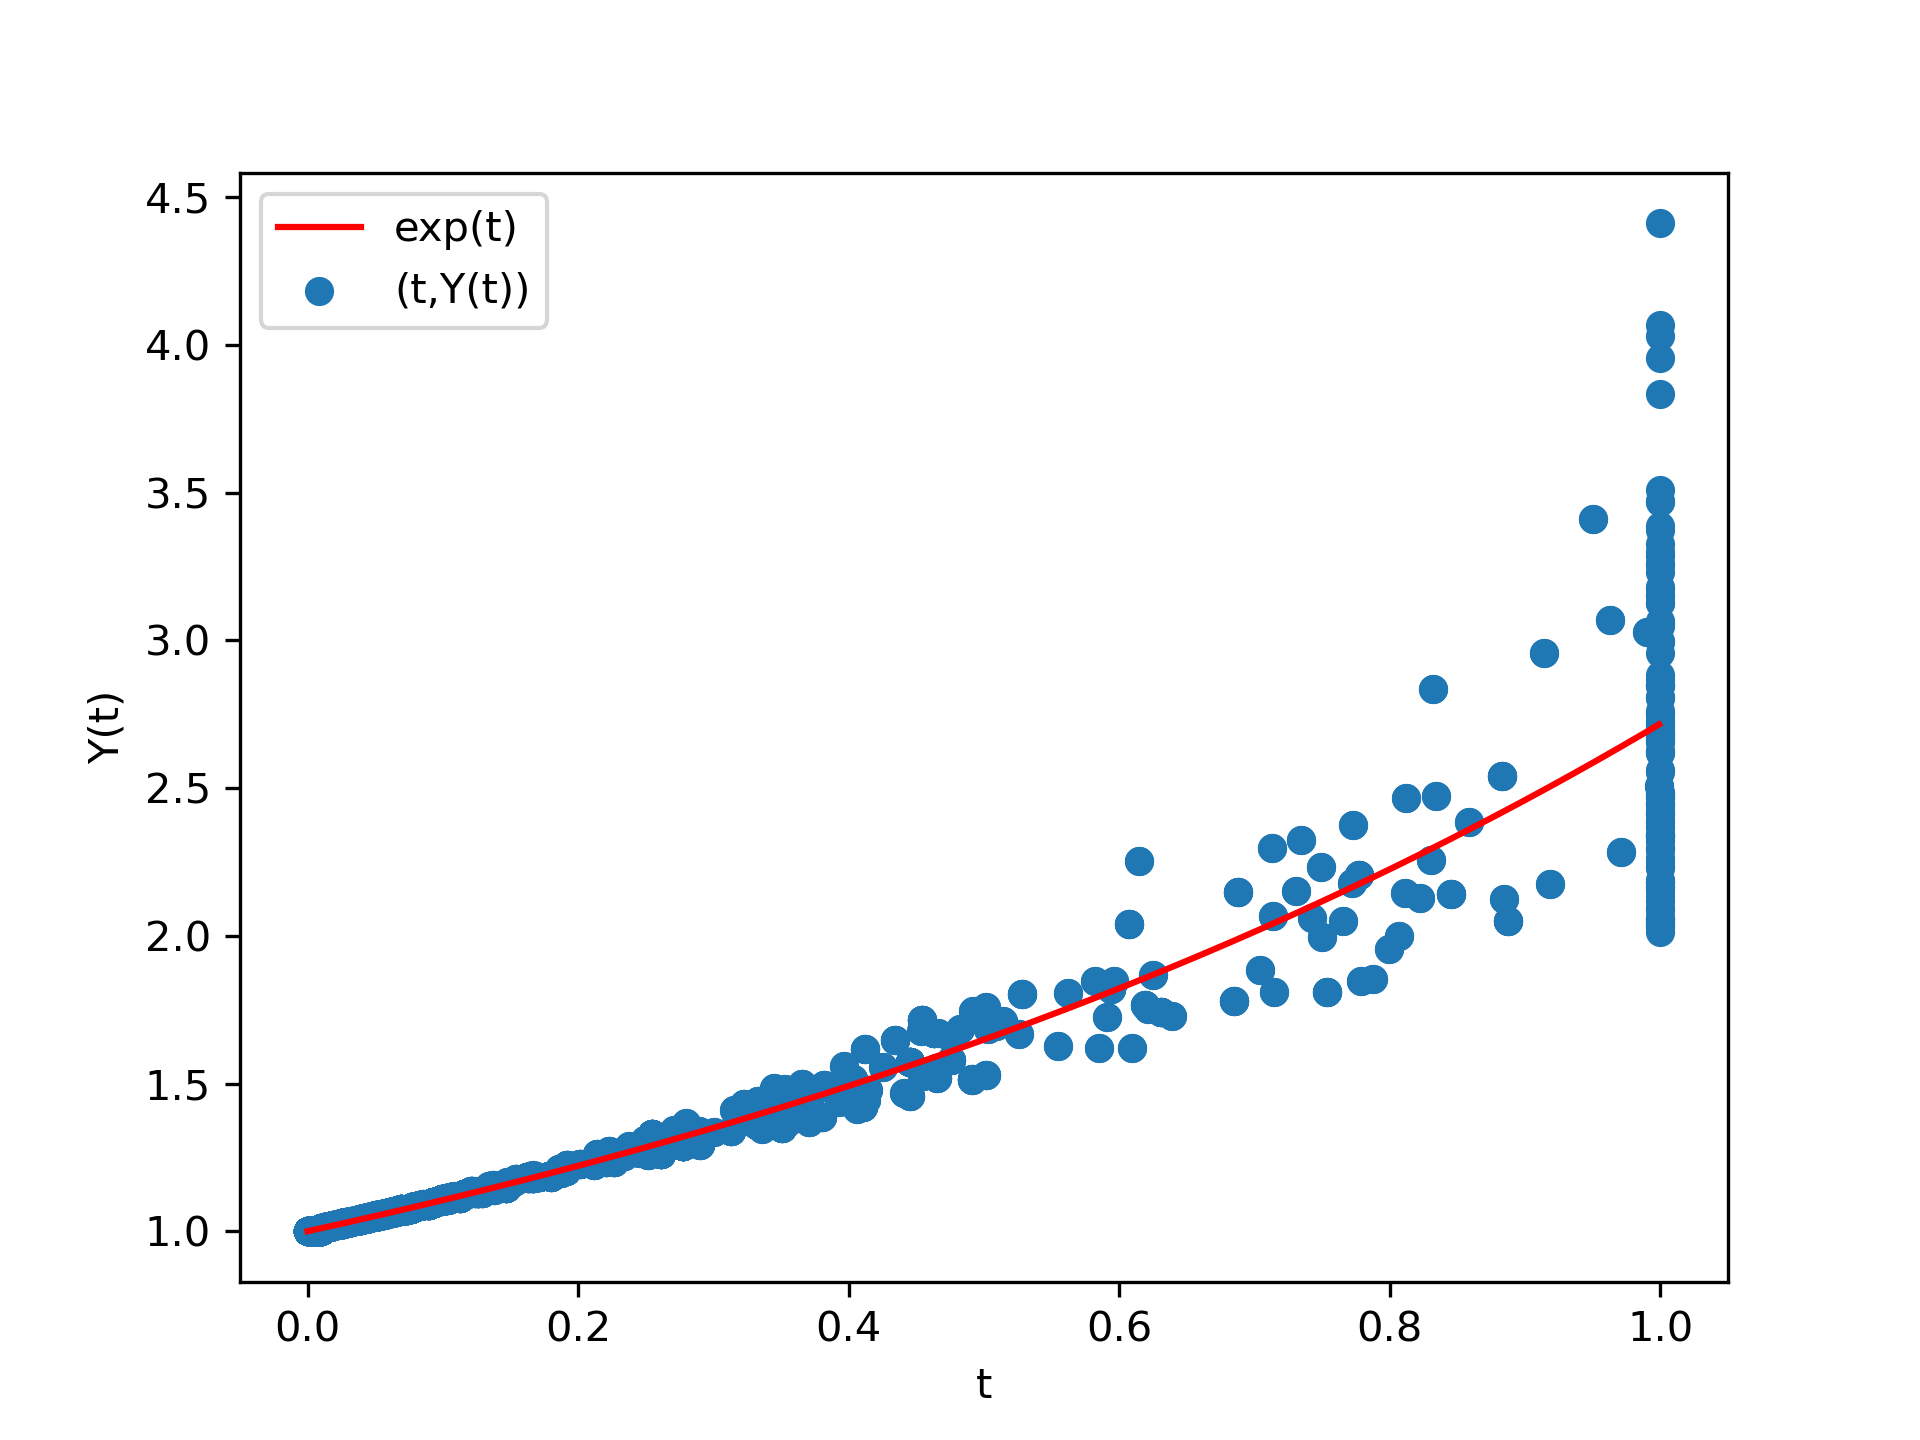
\includegraphics[width=0.8\textwidth]{plots/intro example.png}
        \caption{Recursive calls of (\ref{python eps ydy})}
        \label{fig:intro example}
    \end{figure}
\end{pythonn}

One issue with (\ref{python eps ydy}) is that the variance
increases rapidly as $t$ increases. This issue gets resolved
later (see (\ref{ex:RRMC IVP})). It is important to note that
(\ref{python eps ydy}) retains desirable properties of unbiased Monte
Carlo methods, such as being embarrassingly parallel and having simple
error estimates.

\subsection{Notation}

\textcolor{darkgreen}{
    Maybe it is better to match the notation to recent
    walk on spheres papers. Not sure it is worth it.
} \\

Notations utilized include:
\begin{itemize}
    \item $B(p) \sim \text{Bernoulli}(p) =
              \begin{cases}
                  1 & \text{ if } U<p \\
                  0 & \text{ else }
              \end{cases} $
    \item BVP = Boundary Value Problem
    \item FP = First Passage
    \item $ H(x) =
              \begin{cases}
                  0 & \text{ if } x<0 \\
                  1 & \text{ else }
              \end{cases}$
    \item i.i.d. = independent identically distributed
    \item $U \sim \text{Uniform}(0,1)$
    \item IVP = Initial Value Problem
    \item MC = Monte Carlo
    \item ODE = Ordinary Differential Equation
    \item PDE = Partial Differential Equation
    \item RMC = Recursive Monte Carlo
    \item RRMC = Recursion in Recursion Monte Carlo
    \item RRVE (Recursive Random Variable Equation): An equation that defines a
          family of random variables in terms of itself
    \item RV = Random Variable
    \item Random variables will be denoted with capital letters, e.g., $X$, $Y$ or $Z$.
\end{itemize}

\subsection{Related Work}

\textcolor{darkgreen}{
    There are many papers that we just don't mention because they aren't worth mentioning.
    This video on Youtube \url{https://youtu.be/r8dWZX8IGw8?t=946}
    visualizes related works to covid which is nice to get a broad overview. \\
    Maybe it would also be nice to explain how the primary motivating work and
    the choices that we made have led to the different topics in all sections which
    would explain the cohesion of topics.
} \\

The primary motivating paper for this work is the work
by \citeauthor{sawhney_grid-free_2022}
(\citeyear{sawhney_grid-free_2022}) \cite{sawhney_grid-free_2022},
which introduces the walk-on-sphere method for solving second-order
elliptic PDEs with varying coefficients and Dirichlet boundary conditions.
Their techniques have shown high accuracy even in the presence of geometrically
complex boundary conditions. We focus on the underlying
mechanics of these Monte Carlo techniques.

\begin{related}[MC for IVPs ODEs]
    Monte Carlo methods for initial value problems for systems of ordinary
    differential equations are little studied. The most significant works are:
    \begin{itemize}
        \item \citeauthor{jentzen_random_2009}'s \citeyear{jentzen_random_2009}
              \cite{jentzen_random_2009} paper describes a random Euler scheme for
              weak smoothness conditions.

        \item \citeauthor{daun_randomized_2011}'s \citeyear{daun_randomized_2011}
              \cite{daun_randomized_2011} paper describes a randomized algorithm that
              achieves optimal order of convergence by using polynomial
              extrapolation and control variates.

        \item \citeauthor{ermakov_monte_2019}'s \citeyear{ermakov_monte_2019}
              \cite{ermakov_monte_2019}
              and \citeauthor{ermakov_monte_2021}'s \citeyear{ermakov_monte_2021}
              \cite{ermakov_monte_2021}
              papers study unbiased  methods
              for linear problems and slightly biased methods for nonlinear based
              on Volterra integral equations.

    \end{itemize}


\end{related}

% \begin{related}[MC for linear systems]
%     MC methods can be employed to tackle an ODE or a PDE indirectly
%     by using it on the resulting linear system obtained through
%     a discretization technique. This approach may yield a similar
%     behavior to the original problem. Sampling the Von Neumann series
%     is the primary technique utilized for MC methods in linear systems.

%     \begin{itemize}
%         \item MC methods are common for the page rank problem \cite{zhang_advanced_2021}.
%         \item 
%     \end{itemize}

%     mmm

% \end{related}

% Maybe add a section for the second section?

\subsection{Contributions}
\textcolor{darkgreen}{
    Maybe the discussion of how sections connect or should connect should be done here.
} \\

A significant part of this thesis is dedicated to informally introducing recursive Monte Carlo
with plenty of examples.
The key contribution is an unbiased Monte Carlo method
(\ref{ex:CV RRMC IVP}) for
linear initial value problems for systems of ordinary
differential equations by using recursion in recursion.
This method achieves a higher order of convergence
in the time step size that is comparable to explicit
deterministic methods.



% The key contributions are:

% \begin{itemize}
%     \item Coupled recursion (\ref{ex:coupled recursion}) and
%           recursion in recursion (\ref{tech:recu in recu}) reformulations of
%           ideas that appear in the coupling in
%           \cite{vicini_path_2021} and next flight in
%           rendering see \cite{sawhney_grid-free_2022}
%           the next flight version of walk on sphere.

%     \item An unbiased Monte Carlo method (\ref{ex:CV RRMC IVP}) for
%           linear initial value problems for systems of ordinary
%           differential equations by using recursion in recursion.
%           This method achieves a higher order of convergence
%           in the time step size that is comparable to explicit
%           deterministic methods.

% \end{itemize}

In the background section, we provide an introduction
to Monte Carlo techniques and a short discussion about a Monte Carlo trapezoidal
rule. We also discuss coupled recursion and recursion in recursion. \\

In the ordinary differential equation section, we introduce green functions
as a tool to transform ordinary differential equations into integral equations.
We then proceed to present our main algorithm for solving
linear initial value problems for systems of ordinary differential
equations. \\

In the Brownian motion section, we establish the connection
between Brownian motion and the heat equation using recursive Monte Carlo.
Additionally, we introduce recursive first passage sampling.

\section{Background}

\textcolor{darkgreen}{
    We miss a subsection on stochastcould ic gradient descent (SGD) and
    stochastic variance reduced gradient descent (SVRGD).
    In particular, the connection with ODEs see for example continuous
    gradient descent in \cite{huang_hybrid_2017}. And different ways
    to apply recursion in recursion on SGD which is very similar to
    how we could use recursion in recursion in the next section.
} \\

\subsection{Modifying Monte Carlo}

\textcolor{darkgreen}{
    We didn't add importance sampling because it didn't help and added complexity.
    One thing that we experimented with was how the time of the recursion calls are
    distributed. We like to control this distribution, once it is uniform, it is easy
    to control. We chose a simple Russian roulette that gets the job done for most
    experiments but don't know exactly how the time of the recursion calls are
    distributed in that case. \\
    We have a rough idea but we're not
    sure we can write a proof for it and we still haven't tested it.
    It is importance sampling according
    to a Poisson point process with the right combination of Russian roulette.
    This should make the time of the recursion calls uniformly distributed
    and the amount of recursion calls Poisson distributed. This would simplify
    analyzing the different types of complexities (informational/computational/parallel).\\
} \\

In this subsection, we discuss techniques for modifying RRVEs
in a way that preserves the expected value of the solution while
acquiring more desirable properties. \\

Russian roulette is a MC technique commonly employed in rendering algorithms.
The concept behind Russian roulette is to replace a RV with a
less computationally expensive approximation sometimes.

\begin{definition}[Russian roulette] \label{Russian roulette}
    We define Russian roulette on $X$ with free parameters
    $Y_{1}$, $Y_{2}$ ($E[Y_{1}] = E[Y_{2}]$), $p \in [0,1]$
    and $U$ independent of $Y_{1}$, $Y_{2}$, $X$
    as follows:

    \begin{equation}
        X \rightarrow
        \begin{cases}
            \frac{1}{p}(X - (1-p)Y_{1}) & \text{ if } U < p \\
            Y_{2}                       & \text{ else }
        \end{cases}.
    \end{equation}
\end{definition}

\begin{example}[Russian roulette] \label{ex:simple russian roulette}
    Let us consider the estimation of $E[Z]$, where $Z$ is defined as follows:

    \begin{equation}
        Z = U + \frac{f(U)}{1000}.
    \end{equation}

    Here, $f:\mathbb{R} \rightarrow [0,1]$ is an expensive function to compute.
    Directly estimating $E[Z]$ would involve evaluating $f$ in each simulation,
    which can be computationally costly. To address this, we can modify $Z$ to:

    \begin{equation}
        \tilde{Z} = U + B\left(\frac{1}{100}\right)\frac{f(U)}{10}.
    \end{equation}

    With this modification, $\tilde{Z}$ requires calling $f$ on
    average once every $100$ simulations, significantly reducing the
    computational burden compared to simulating $Z$. Although the variance of $\tilde{Z}$
    increases slightly compared to $Z$, it is more efficient.

\end{example}

\begin{related}[Russian roulette]
    For example (\ref{ex:simple russian roulette}) it is possible to estimate
    the expectance of the $2$ terms of $Z$ separately. Given the variances and
    computational complexity of both terms, you can calculate the asymptotic optimal
    division of samples for each term. \\
    In \cite{rath_ears_2022} they approximate optimal Russian roulette and splitting
    (RRS) factors with fixed-point iterations to maximize the efficiency of a renderer.
\end{related}

\begin{example}[Russian roulette on (\ref{recursive RV})] \label{ex: russian roulette}
    To address the issue of indefinite recursion in equation
    (\ref{recursive RV}), Russian roulette can be employed
    by approximating the value of $Y$ near $t = 0$ with $1$
    sometimes. Specifically, we replace the coefficient $t$
    in front of the recursive term with $B(t)$ when $t < 1$.
    The modified recursive expression for $Y(t)$ becomes:

    \begin{equation}
        Y(t) =
        \begin{cases}
            1 + B(t)Y(Ut) & \text{ if } t < 1 \\
            1 + tY(Ut)    & \text{ else}
        \end{cases}.
    \end{equation}
\end{example}

\vspace{0.2cm}

\begin{pythonn}[implementation of (\ref{ex: russian roulette})] \label{RRpython}
    \pythoncode{python code/RR_ydy.py}
    Interestingly, $\forall t \le 1:Y(t)$ is constrained to take on only integer values.
    This is visually clear in Figure \ref{fig:russian roulette}.
    \begin{figure}[h!]
        \centering
        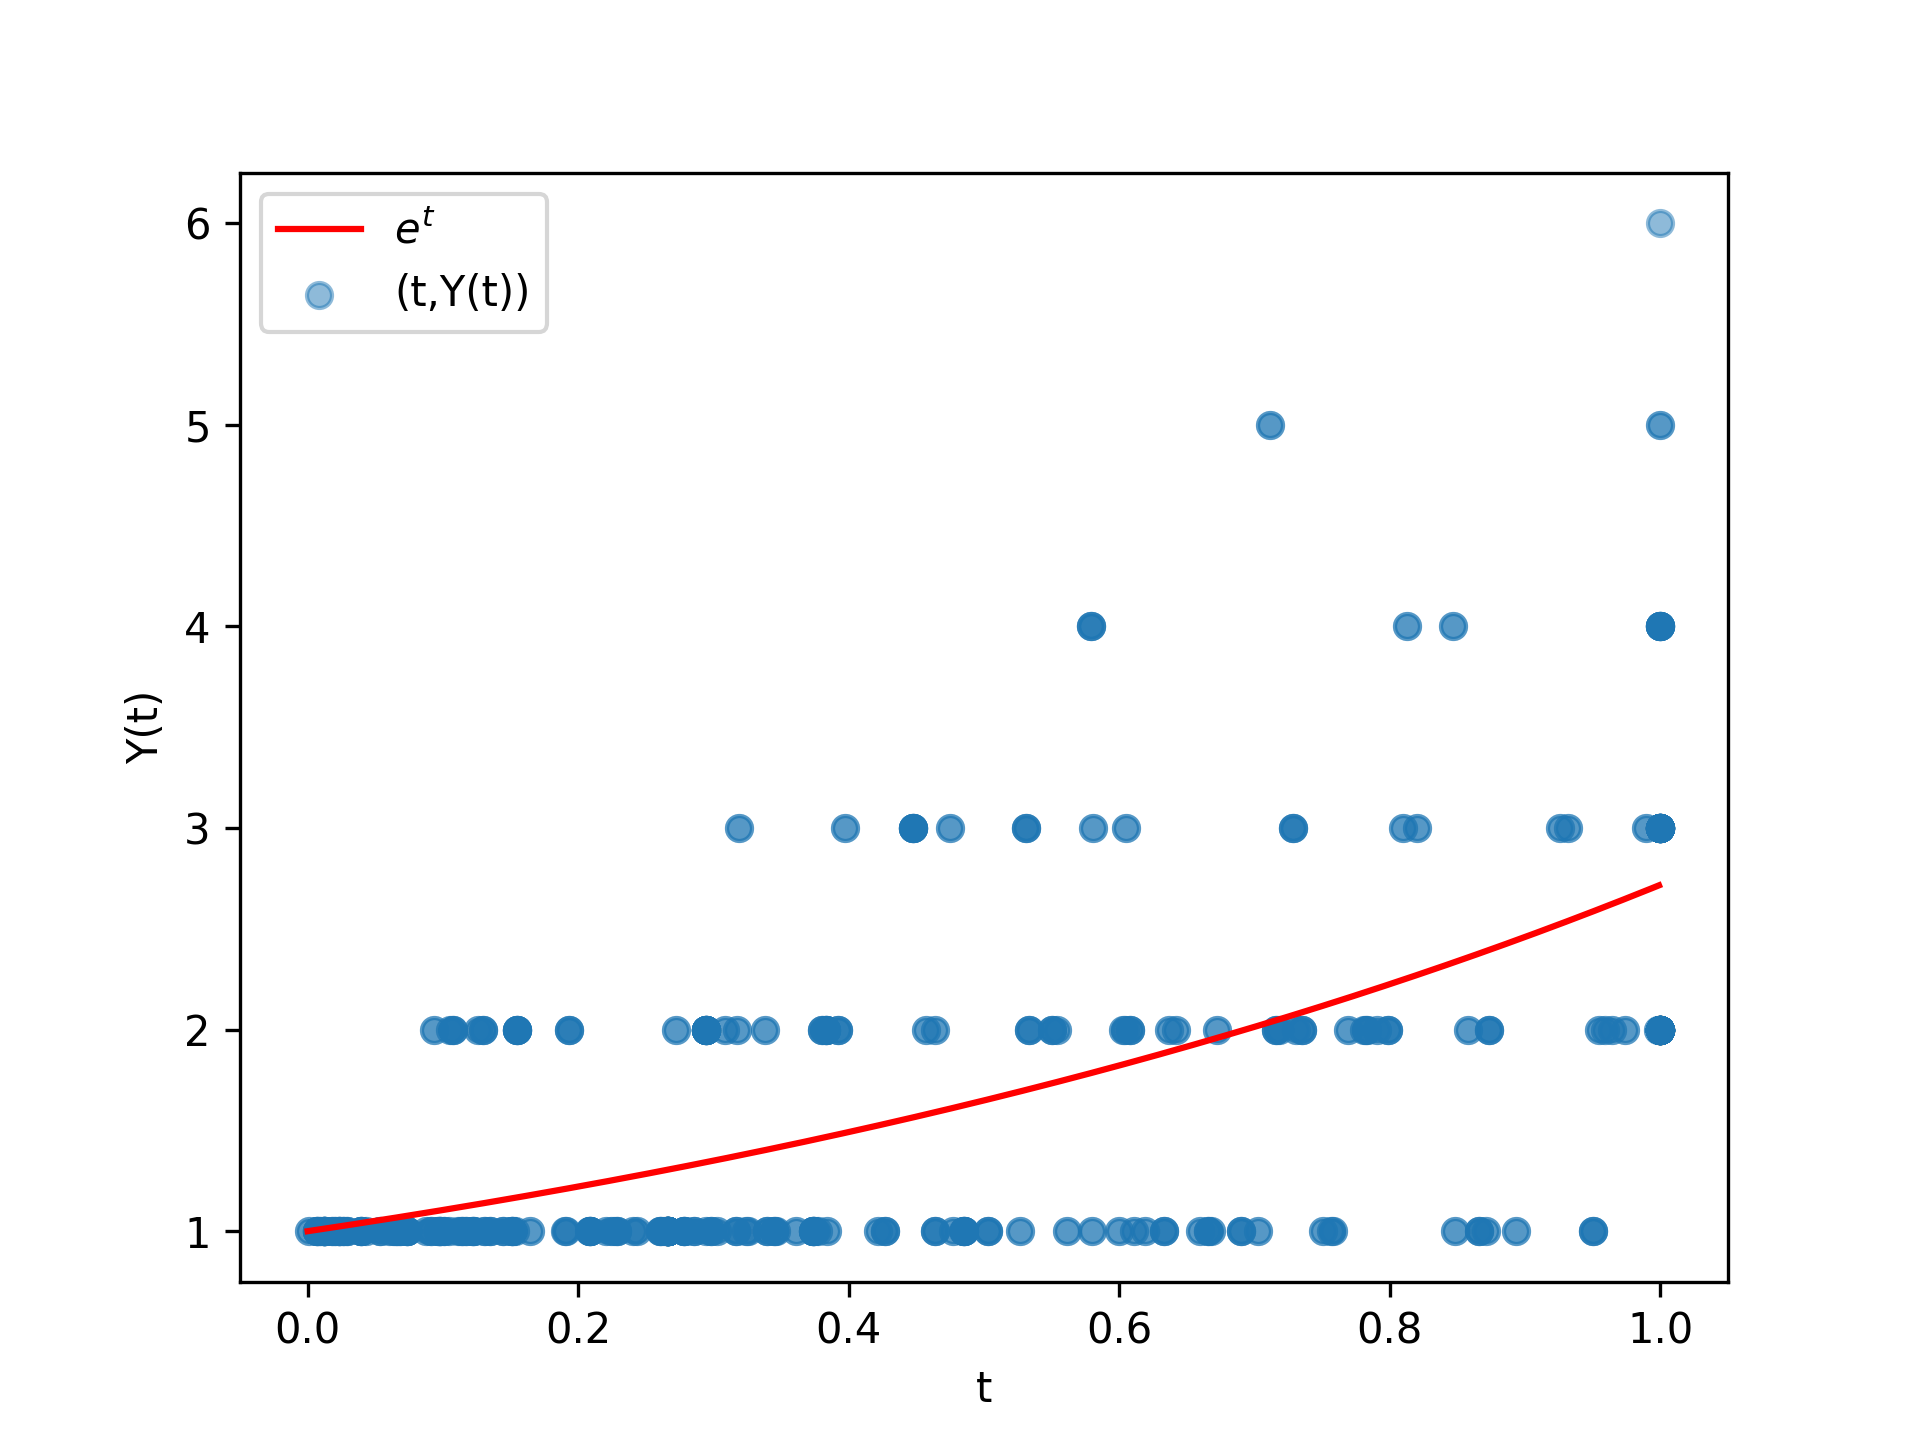
\includegraphics[width=0.8\textwidth]{plots/russian roulette example.png}
        \caption{Recursive calls $(t,Y(t))$ of (\ref{RRpython}) }
        \label{fig:russian roulette}
    \end{figure}

\end{pythonn}

Splitting is a technique that has almost the reverse effect of Russian roulette.
Instead of reducing the number of simulations of a RV as Russian roulette does,
we increase it by using more samples (i.e., splitting the sample) which
reduces the variance.

\begin{definition}[splitting] \label{def:splitting}
    Splitting $X$ refers to utilizing multiple $X_{j} \sim X$ (not necessarily independent) to
    reduce variance by taking their average:
    \begin{equation}
        \bar{X} = \frac{1}{N} \sum_{j=1}^{N} X_{j}.
    \end{equation}
\end{definition}

Splitting the recursive term in a RRVE can result in additive branching recursion,
necessitating cautious management of terminating the branches promptly to prevent
exponential growth in computational complexity. To accomplish this, termination
strategies that have been previously discussed can be employed. Subsequently,
we will explore the utilization of coupled recursion as a technique to mitigate
additive branching recursion in RRVEs (refer to (\ref{ex:coupled splitting})).

\begin{example}[splitting on (\ref{recursive RV})] \label{ex:splitting}
    We can "split" the recursive term of Equation (\ref{recursive RV})
    into two parts as follows:

    \begin{equation}
        Y(t) = 1 + \frac{t}{2}(Y_{1}(Ut) + Y_{2}(Ut)),
    \end{equation}

    where $Y_{1}(t)$ and $Y_{2}(t)$ are i.i.d. with $Y(t)$.
\end{example}

\vspace{0.2cm}

\begin{pythonn}[implementation of (\ref{ex:splitting})]
    \pythoncode{python code/SRR_ydy.py}
\end{pythonn}

% \begin{definition}[$2$-level MC] \label{2 level}
%     $2$-level MC on $X$ with parameters $\tilde{X}, Y: E[\tilde{X}]=E[Y]$:
%     \begin{equation}
%         X \rightarrow X-\tilde{X} + Y.
%     \end{equation}
% \end{definition}

\begin{definition}[control variates] \label{CV}
    Define control variating $f(X)$ with $\tilde{f}$ an approximation of $f$ as:
    \begin{equation}
        f(X) \rightarrow (f-\tilde{f})(X) + E[\tilde{f}(X)].
    \end{equation}

    Note that control variating requires the evaluation of
    $E[\tilde{f}(X)]$. When this is estimated instead of evaluated
    exactly, we refer to it as $2$-level MC.
\end{definition}


\begin{example}[control variate on (\ref{recursive RV})] \label{ex:CV}
    To create a control variate for Equation (\ref{recursive RV}) that
    effectively reduces variance, we employ the approximation
    $y(t) \approx 1+t$ and define the modified recursive term as follows:

    \begin{equation}
        Y(t) = 1 + t + \frac{t^2}{2} + t(Y(Ut) - 1 - Ut).
    \end{equation}

    It is important to note that while we could cancel out the constant term
    of the control variate, doing so would have a negative impact on
    the Russian roulette implemented later.
\end{example}

\vspace*{0.2cm}
\begin{pythonn}[implementation of (\ref{ex:CV})]
    \pythoncode{python code/CVRR_ydy.py}
\end{pythonn}

\begin{related}[MC modification]
    Our favorite work that discusses these techniques is \cite{veach_robust_1997}.
    More interesting MC techniques can be found in rendering.
    % $2$-level gets discussed in \cite{giles_multilevel_2013} a introductory paper to
    % multilevel MC.
\end{related}
% need to fix veach reference see bibliography

\subsection{Monte Carlo Trapezoidal Rule}

\textcolor{darkgreen}{
    When working on this section we had a vague notion of information complexity
    which corresponds to statistical complexity we do know from a
    statical learning course from CMU \cite{ryan_t_lecture_2017}.
    This subsection misses vital references and results (with definitions) of
    information complexity of integration for different
    measures of errors, the curse of dimensionality, what this implies
    for harder problems than integration and the limitations of this way
    of analyzing algorithms or methods.  We like the chapter on
    the curse of dimensionality in
    \cite{foucart_mathematical_2022}.
    Quantum information complexity is only slightly better than
    random information complexity (roughly a quadratic improvement)
    \cite{heinrich_optimal_2001}.
    \\
    We also love to add methods that
    exploit smoothness but we aren't comfortable with them.
    We like the book that \citeauthor{trefethen_approximation_nodate}
    (also the author of chebfun package in matlab)
    wrote \cite{trefethen_approximation_nodate} on
    chebychev polynomial things.
} \\

In this subsection, we introduce a MC trapezoidal rule that
exhibits similar convergence behavior to the methods discussed later.
The MC trapezoidal rule is essentially a regular Monte Carlo method
enhanced with control variates based on the trapezoidal rule.

\begin{definition}[MC trapezoidal rule]
    We define the MC trapezoidal rule for approximating the integral
    of function $f$ over the interval $[x, x+\Delta x]$ with a Russian roulette rate
    $l$ and $\tilde{f}$ the linear approximation of $f$ corresponding
    to the trapezoidal rule as follows:

    \begin{align}
         & \int_{x}^{x+\Delta x} f(s) ds                                       \\
         & = \int_{x}^{x+\Delta x}  \tilde{f}(s) ds +
        \int_{x}^{x+\Delta x}  f(s) - \tilde{f}(s) ds                          \\
         & = \Delta x \frac{f(x) + f(x+\Delta x)}{2}
        + E \left[l B\left( \frac{1}{l}\right)(f(S_x) - \tilde{f}(S_x))\right] \\
         & \approx \Delta x \frac{f(x) + f(x+\Delta x)}{2}                     \\
         & + \Delta x l B\left( \frac{1}{l}\right)
        \left(f(S_x) - f(x) - \frac{S_x - x}{\Delta x}
        \left(f(x+\Delta x) - f(x)\right) \right),
    \end{align}

    where $S_x \sim \text{Uniform}(x,x+\Delta x)$.
\end{definition}


This MC trapezoidal rule has on average $\frac{1}{l}$ more function calls than
the normal trapezoidal rule. For the composite rule with $n$ intervals,
there are $\text{Binomial}(n,\frac{1}{l})$ additional function calls.

% The composite MC trapezoidal rule, defined as the sum of MC trapezoidal rules
% on equally divided intervals, can be computationally expensive. Each interval
% requires an additional function call compared to the regular composite MC
% trapezoidal rule. However, by aggressively applying Russian roulette into
% the normal trapezoidal rule, the increase in function calls can be made
% arbitrarily small.

\begin{definition}[composite MC trapezoidal rule] \label{MCtrap}
    Define the composite MC trapezoidal rule for approximating the integral
    of function $f$ over the interval $[a, b]$ with $n$ intervals
    and a Russian roulette rate $l$ as follows:

    \begin{align}
        \int_{a}^{b} f(s) ds \approx \Delta x \sum_{x} & \frac{f(x) + f(x+\Delta x)}{2} \\
                                                       & + l B\left(\frac{1}{l}\right)
        \left(f(S_x) - f(x) - \frac{S_x - x}{\Delta x}(f(x+\Delta x) - f(x))\right),
    \end{align}

    where $S_x \sim \text{Uniform}(x,x+\Delta x)$.

\end{definition}

\begin{pythonn}[implementation of (\ref{MCtrap})]
    We implement (\ref{MCtrap}) for $\int_{0}^{1}e^{s}ds$.
    \vspace*{0.5cm}
    \pythoncode{python code/trap1.py}

    \begin{figure}[h!]
        \centering
        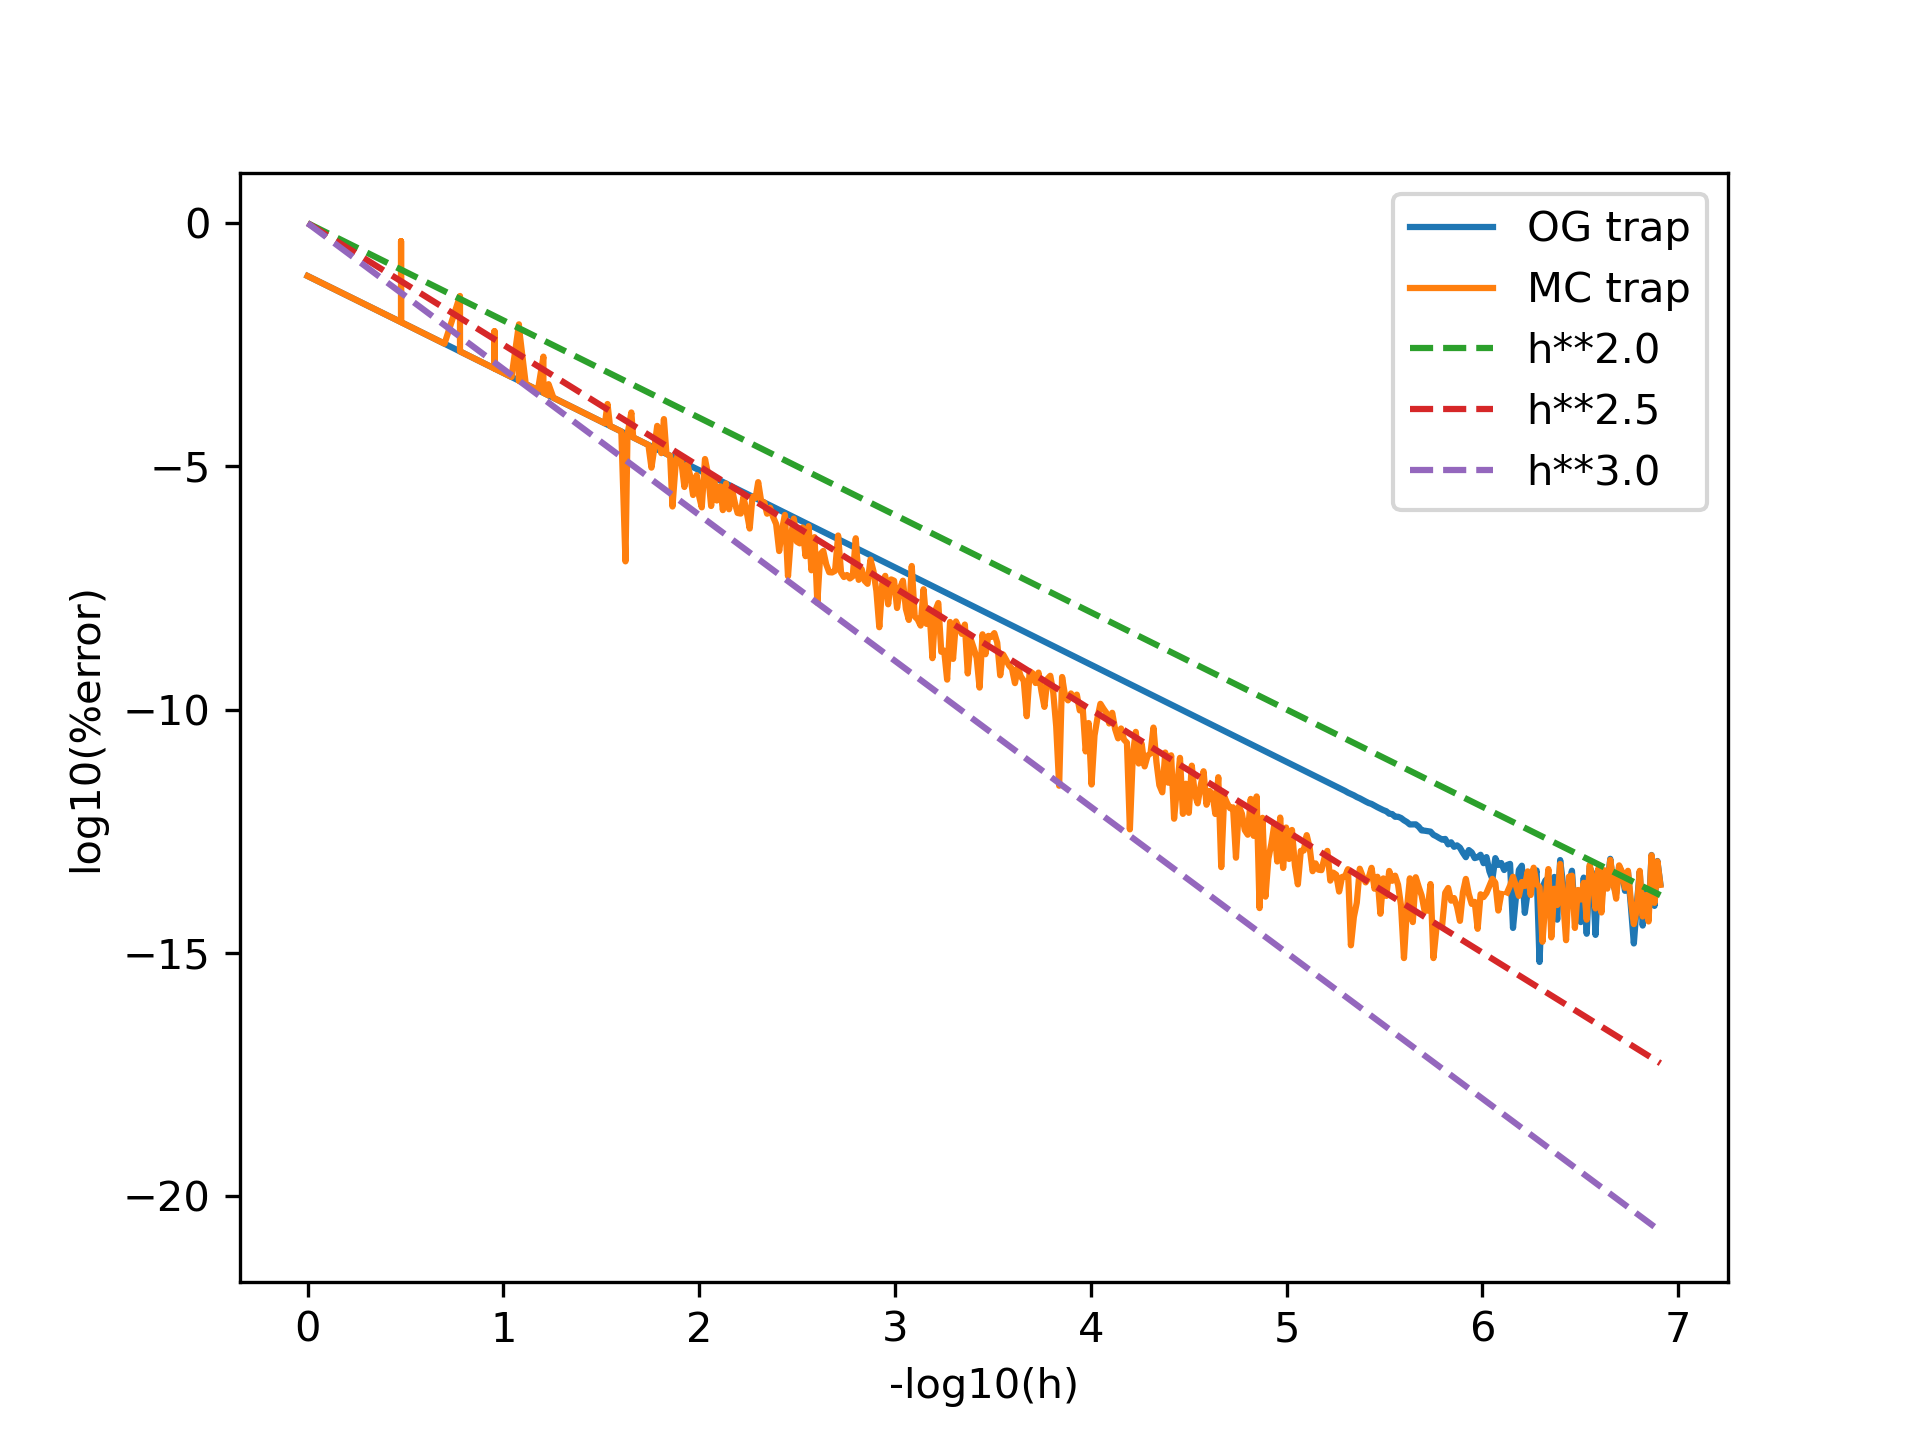
\includegraphics[width=0.8\textwidth]{plots/MCtrap.png}
        \caption{Log-log plot of the error of (\ref{MCtrap}) for
        $\int_{0}^{1}e^{s}ds$ with $l=100$ at which the additional function
        calls are negligible. At floating point accuracy,
        the convergence ceases.
        }
        \label{fig:MCtrap}
    \end{figure}
\end{pythonn}

We postulate that this MC composite rule enhances the convergence
rate by $0.5$ orders compared to the standard composite rule for each dimension,
provided that the appropriate conditions of smoothness are met.
To substantiate this conjecture, we shall outline our rationale concerning
the accumulation of unbiased polynomial errors.\\

For the sake of simplicity, we reduce the study of the local truncation error
to the following expression:
\begin{equation}
    \int_{0}^{h} s^{2}ds = O(h^{3}).
\end{equation}

In the standard composite rule, we would drop this term, but in
the MC version, we eliminate the bias. As a result,
the local truncation error behaves similarly to:

\begin{equation}
    \int_{0}^{h} s^{2}ds- h(hU)^{2} = \int_{0}^{h} s^{2}ds- h^{3}U^{2} = O(h^{3}).
\end{equation}

The main distinction between the standard and MC rule lies in how they
accumulate local truncation errors into global truncation error. In the standard
case, there is a loss of one order. When measuring the error of randomized algorithms,
the root-mean-square error is typically used, which, in the unbiased case,
is equivalent to the standard deviation:

\begin{align}
    \sqrt{\text{Var}\left(\sum_{j=1}^{n} \int_{0}^{h} s^{2}ds- h^{3}U_{j}^{2}\right)}
     & =\sqrt{\text{Var}\left(\sum_{j=1}^{n} h^{3}U_{j}^{2}\right)}   \\
     & =h^{3} \sqrt{\text{Var}\left( \sum_{j=1}^{n} U_{j}^{2}\right)} \\
     & =h^{3} \sqrt{ \sum_{j=1}^{n}\text{Var} (U_{j}^{2})}            \\
     & =h^{3} \sqrt{ n \text{Var}(U^{2})}                             \\
     & =h^{3} \sqrt{n} \sqrt{ \text{Var}(U^{2})}                      \\
     & = O(h^{2.5}).
\end{align}

Note that the meaning of a bound on the error that behaves as $O(h^{2})$ and
a bound on the root-mean-square error that behaves as $O(h^{2})$ is different.
A bound on the error implies a bound on the root-mean-square error, but
the reverse is not true.

\subsection{Unbiased Non-Linearity}

\textcolor{darkgreen}{
    Missed an important paper of Nvidia for estimating
    transmittance \cite{kettunen_unbiased_2021}
    which is just example \ref{ex:exp int} but efficient.
    It needs to be extended to matrix exponentials
    this opens the path to exponential integrator
    methods \cite{hochbruck_exponential_2010} or maybe even methods
    that directly estimate the magnus expansion. \\
    Example \ref{ex:nonlinear example} is a bad example
    to study RMC because it is too nice. \\
    Controlling the distribution of the time of the recursion calls
    is even harder with branching. The way to extend our idea with the Poisson
    process is to divide the expected 'intensity' over the branches.
} \\

In this subsection, we present techniques for handling non-linearity.
It may appear that unbiased approaches are only applicable to linear
problems. By utilizing independent samples, it becomes possible to handle
polynomial non-linearities.

While transforming non-linearities into polynomials may not always be straightforward,
it is still possible to develop biased alternative approaches based on linearization
or approximate polynomial non-linearities.


\begin{example}[$y'=y^{2}$] \label{ex:nonlinear example}
    Consider the following ODE:

    \begin{equation} \label{eq:nonlinear example}
        y' = y^2, \quad y(1) = -1.
    \end{equation}

    The solution to this equation is given by $y(t) = -\frac{1}{t}$.
    By integrating both sides of equation (\ref{eq:nonlinear example}),
    we obtain the following integral equation:

    \begin{equation}
        y(t) = -1 + \int_{1}^{t} y(s) y(s)ds.
    \end{equation}

    To estimate the recursive integral in equation (\ref{eq:nonlinear example}),
    we use i.i.d. $Y_1,Y_2 \sim Y$ in following RRVE:

    \begin{equation} \label{RRVE: nonlinear example}
        Y(t) = -1 + (t-1) Y_1(S) Y_2(S),
    \end{equation}

    where $S \sim \text{Uniform}(1,t)$.
    Branching RRVEs are typical when dealing
    with non-linearity.
\end{example}

\vspace*{0.2cm}
\begin{pythonn}[implementation (\ref{ex:nonlinear example})]\label{py:nonlinear example}
    %important note while implementing equation (\ref{RRVE yy2})  
    \pythoncode{python code/dyy2.py}
    In this implementation $Y(t)$ only takes values $\{-1,0\}$.
\end{pythonn}

\begin{example}[$e^{E[X]}$] \label{ex:exp int}
    $e^{\int x(s)ds}$ is a common expression encountered when studying ODEs.
    In this example, we demonstrate how you can generate unbiased estimates of
    $e^{E[X]}$ with simulations of $X$. The Taylor series of $e^{x}$ is:
    \begin{align}
        e^{E[X]} & = \sum_{n=0}^{\infty} \frac{E^{n}[X]}{n!}     \\
                 & = 1 + \frac{1}{1}E[X]\left(1+ \frac{1}{2}E[X]
        \left(1+\frac{1}{3}E[X]\left(1+ ...\right)\right)\right). \label{taylor e}
    \end{align}
    Change the fractions of equation (\ref{taylor e}) to Bernoulli processes
    and replace all $X$ with independent $X_j$ with $E[X]=E[X_{i}]$.
    \begin{align}
        e^{E[X]} & = E
        \left[1 + B\left(\frac{1}{1}\right)E[X_1]
        \left(1+ B\left(\frac{1}{2}\right)E[X_2]
        \left(1+B\left(\frac{1}{3}\right)E[X_3]
        \left(1+ ...\right)
        \right)
        \right)
        \right]              \\
                 & = E\left[
            1 + B\left(\frac{1}{1}\right)X_1
            \left(1+ B\left(\frac{1}{2}\right)X_2
            \left(1+B\left(\frac{1}{3}\right)X_3
            \left(1+ ...\right)
            \right)
            \right)
            \right]
    \end{align}
    What is inside the expectation is something that we can simulate with simulations of $X_{j}$.
\end{example}

\vspace{0.2cm}
\begin{pythonn}[implementation of $e^{E[X]}$ (\ref{ex:exp int})]
    The following python code estimates $e^{\int_{0}^{t} s^{2}ds}$:
    \vspace*{0.4cm}
    \pythoncode{python code/expX.py}
    %}
\end{pythonn}

\begin{related}[unbiased non-linearity]
    A similar approach to non-linearity can be found in \cite{ermakov_monte_2019}.
\end{related}

\subsection{Recursion}

\textcolor{darkgreen}{
    We should add alternatives to tail recursion and discuss them.
    These do get discussed in our Python notebooks but
    we thought that tail recursion would be sufficient.
    We noticed later that for big matrices it is more efficient to
    execute first the matrix-vector (without any strong unbiased
    approximations) products. This is clear in example \ref{ex:tail on couple}
    on line 7 and 8.
} \\
In this subsection, we discuss recursion-related techniques.

\begin{technique}[coupled recursion]
    The idea behind coupled recursion is sharing recursion calls of
    multiple RRVEs for simulation. This does make them dependent.
    % It is like assuming $2$ induction hypotheses at the same
    % time and proving both inductions steps at the same time vs
    % doing separate induction proofs. Which should be easier
    % because you have access to more assumptions at the same time.
\end{technique}

\begin{example}[coupled recursion] \label{ex:coupled recursion}
    Consider calculating the
    sensitivity of following ODE to a
    parameter $a$:
    \begin{align}
        y'             & =ay,y(0)=1 \Rightarrow \label{couple recu ex1} \\
        \partial_{a}y' & = y + a \partial_{a}y \label{couple recu ex2}
    \end{align}
    Turn (\ref{couple recu ex1}) and (\ref{couple recu ex2}) into RRVEs.
    To emphasize that they are coupled, that they should
    recurse together we write them in a matrix equation:
    \begin{equation} \label{coupled mat}
        \begin{bmatrix}
            Y(t) \\
            \partial_{a}Y(t)
        \end{bmatrix}=
        X(t)=
        \begin{bmatrix}
            1 \\
            0
        \end{bmatrix}+
        t \begin{bmatrix}
            a & 0 \\
            1 & a
        \end{bmatrix}
        X(Ut).
    \end{equation}

    Observe how this eliminates the additive branching recursion
    present in equation (\ref{couple recu ex2}).

\end{example}

\begin{pythonn} [implementation of (\ref{coupled mat})]
    \pythoncode{python code/coupled_mat.py}
\end{pythonn}

\begin{related}[coupled recursion]
    Example (\ref{ex:coupled recursion}) is inspired by \cite{vicini_path_2021}.
    \cite{vicini_path_2021} propose an efficient unbiased backpropagation
    algorithm for rendering.
    \cite{yilmazer_solving_2022} extends \cite{vicini_path_2021} to walk on spheres.
    % Coupling feels close to percolation \cite{duminil-copin_sixty_2019}.
    % Maybe I should search a paper that coupling in happens
\end{related}

\begin{technique}[recursion in recursion]\label{tech:recu in recu}
    Recursion in recursion is like proving an induction
    step of an induction proof with induction. Recursion in recursion
    uses an inner recursion in the outer recursion.
\end{technique}

\begin{related}[recursion in recursion]
    Beautiful examples of recursion in recursion are
    the next flight variant of WoS in
    \cite{sawhney_grid-free_2022} and epoch-based algorithms in optimization
    \cite{gupta_convergence_2021}.
\end{related}

Most programming languages do support recursion, but it often comes with certain
limitations such as maximum recursion depth and potential performance issues.
When applicable, tail recursion can be used to
implement recursion that addresses these concerns.

\begin{technique}[non-branching tail recursion]
    Tail recursion involves reordering all operations
    so that almost no operation needs to happen after
    the recursion call. This allows us to return the
    answer without retracing all steps when we reach
    the last recursion call and it can achieve similar
    speeds to a forward implementation.
\end{technique}

The non-branching recursion presented in the RRVEs
can be implemented with tail recursion due to the associativity of
all operations ($(xy)z = x(yz)$) involved. However, tail recursion
may not always be desirable as it discards intermediate values of
the recursion calls which may be of interest. To retain some of these intermediate
values while still partly optimizing for performance, it is possible
to combine tail recursion with normal recursion.

\begin{pythonn}[tail recursion on (\ref{coupled mat})] \label{ex:tail on couple}
    We implement (\ref{coupled mat}) but this time with tail recursion.
    We collect addition operations in a vector $sol$ and multiplication
    in a matrix $W$. $W$ may be referred to as accumulated weight or throughput.
    \vspace{0.3cm}
    \pythoncode{python code/tailrecu.py}
\end{pythonn}


\subsection{Limitations and Future Work}

\textcolor{darkgreen}{
    Don't know what to do with this subsection. Maybe it is better to call it
    intrestring things that we didn't use yet.
} \\

There are several MC techniques we did not discuss like quasi-MC and importance sampling.
We would like to mention SALT  a MC technique that we find
particularly interesting and has received relatively little attention.

\begin{technique}[SALT]
    Sequential Approximation in L-Two (SALT) is an adaptive MC technique
    that builds control variates with a (bi-)orthonormal basis. The
    rough idea behind it is that calculating coefficients for
    a (bi-)orthonormal basis can be found by MC integration and
    the current estimate of those coefficients can accelerate MC integration.
    It can be seen as an interesting case of stochastic gradient descent.
\end{technique}

% \begin{example}[SALT wavelet]
%     check period 3
% \end{example}

\begin{related}[SALT]
    SALT gets discussed in \cite{gobet_new_2014}. Other noteworthy papers on
    adaptive MC techniques are \cite{he_adaptive_2021} on adaptive important sampling
    and \cite{salaun_regression-based_2022} on regression-based MC.
\end{related}

% improving (\ref{ex:exp int})

\begin{related}[MC trapezoidal rule]
    In \cite{wu_randomised_2020}, an improvement of half
    order for a MC trapezoidal rule is discussed. We are
    uncertain whether this improvement is similar to ours.
    Further examination would be needed.
\end{related}

Our current method for handling non-linearity, as demonstrated
in (\ref{ex:exp int}), is rudimentary and only applicable to small
levels of non-linearity. We have not tested any
variance reduction techniques in this context. We think that
major improvements can be made in (\ref{ex:exp int}). \\
% \begin{example}[fixpoint]
%     check period 1
% \end{example}


We did not discuss branching tail recursion but
it is important to improve our approach to handling non-linearity.
There exist multiple methods of implementing branching tail recursion,
each with its own set of benefits and drawbacks.
% When it comes to recursive
% MC, tree regrowing is particularly noteworthy.

\begin{technique}[checkpointing]
    The structure of branching recursion can be captured by a tree. Storing that tree
    in memory can be expensive. In recursion, you only need to retrace steps
    $1$ by $1$ therefore you only need local parts of the recursion tree.
    Checkpointing tries to alleviate memory issues by instead storing the whole
    tree only storing seeds (of the random generator) of parts of the
    tree and growing them when needed.
\end{technique}


\begin{related}[branching tail recursion]
    Checkpointing appears in
    \cite{vicini_path_2021}.
    % This blog discusses branching tail recursion:
    % \url{https://jeroenvanwijgerden.me/post/recursion-1/}.
\end{related}

\section{Ordinary Differential Equations}

%\subsection{Linear Recursive Integrals}
%We have an lgorithm in mind for this case based on coupled recursion on disjunct sets.
%
%\begin{definition}[Volterra equation of the second kind]
%    A Volterra equation of the second kind for $x$  is of the following form:
%    $$
%        x(t)=f(t)+\int_a^t K(t, s) x(s) ds.
%    $$
%    Given the kernel  $K(t, s)$  and  $ f(t)$.
%\end{definition}
%


\subsection{Green Functions}

\textcolor{darkgreen}{
    This section better goes in the background section. We just need
    green functions defined.
} \\

In this subsection, we discuss informally how to turn ODEs into integral equations mainly
by example. Our main tool for this are green functions.
Prior to discussing green functions, we offer several
examples.

\begin{example}[$y'=y$ average condition]
    We will solve the equation:

    \begin{equation} \label{ydy int}
        y' = y,
    \end{equation}

    but this time with a different condition:

    \begin{equation}
        \int_{0}^{1} y(s) ds = e-1.
    \end{equation}

    The solution to this equation remains the same: $y(t) = e^{t}$.
    We define the corresponding source green function $G(t,x)$ for $y'$
    and this type of condition as follows:

    \begin{equation}
        G' = \delta(x-t), \quad \int_{0}^{1} G(s,x) ds = 0.
    \end{equation}

    Solving this equation yields:

    \begin{equation}
        G(t,x) = H(t-x) + x - 1.
    \end{equation}

    It is worth noting that we could have chosen a different
    green function corresponding to a different linear
    differential operator.

    At this point, it may not be clear, but using this green function,
    we can form the following integral equation for (\ref{ydy int}):

    \begin{equation} \label{int ydy int}
        y(t) = e - 1 + \int_{0}^{1} G(t,s) y(s) ds.
    \end{equation}

    Converting equation (\ref{int ydy int}) into a RRVE
    using RMC, we obtain:

    \begin{equation}\label{RRVE ydy int}
        Y(t) = e - 1 + 2B\left(\frac{1}{2}\right)Y(S)(H(t-S)+S-1),
    \end{equation}

    where $S \sim U$. We will skip the Python implementation
    of equation (\ref{RRVE ydy int}) as it does not provide any
    new information. Instead, we will plot realizations of
    equation (\ref{RRVE ydy int}) in Figure \ref{fig:ydy int}.

    \begin{figure}[h!]
        \centering
        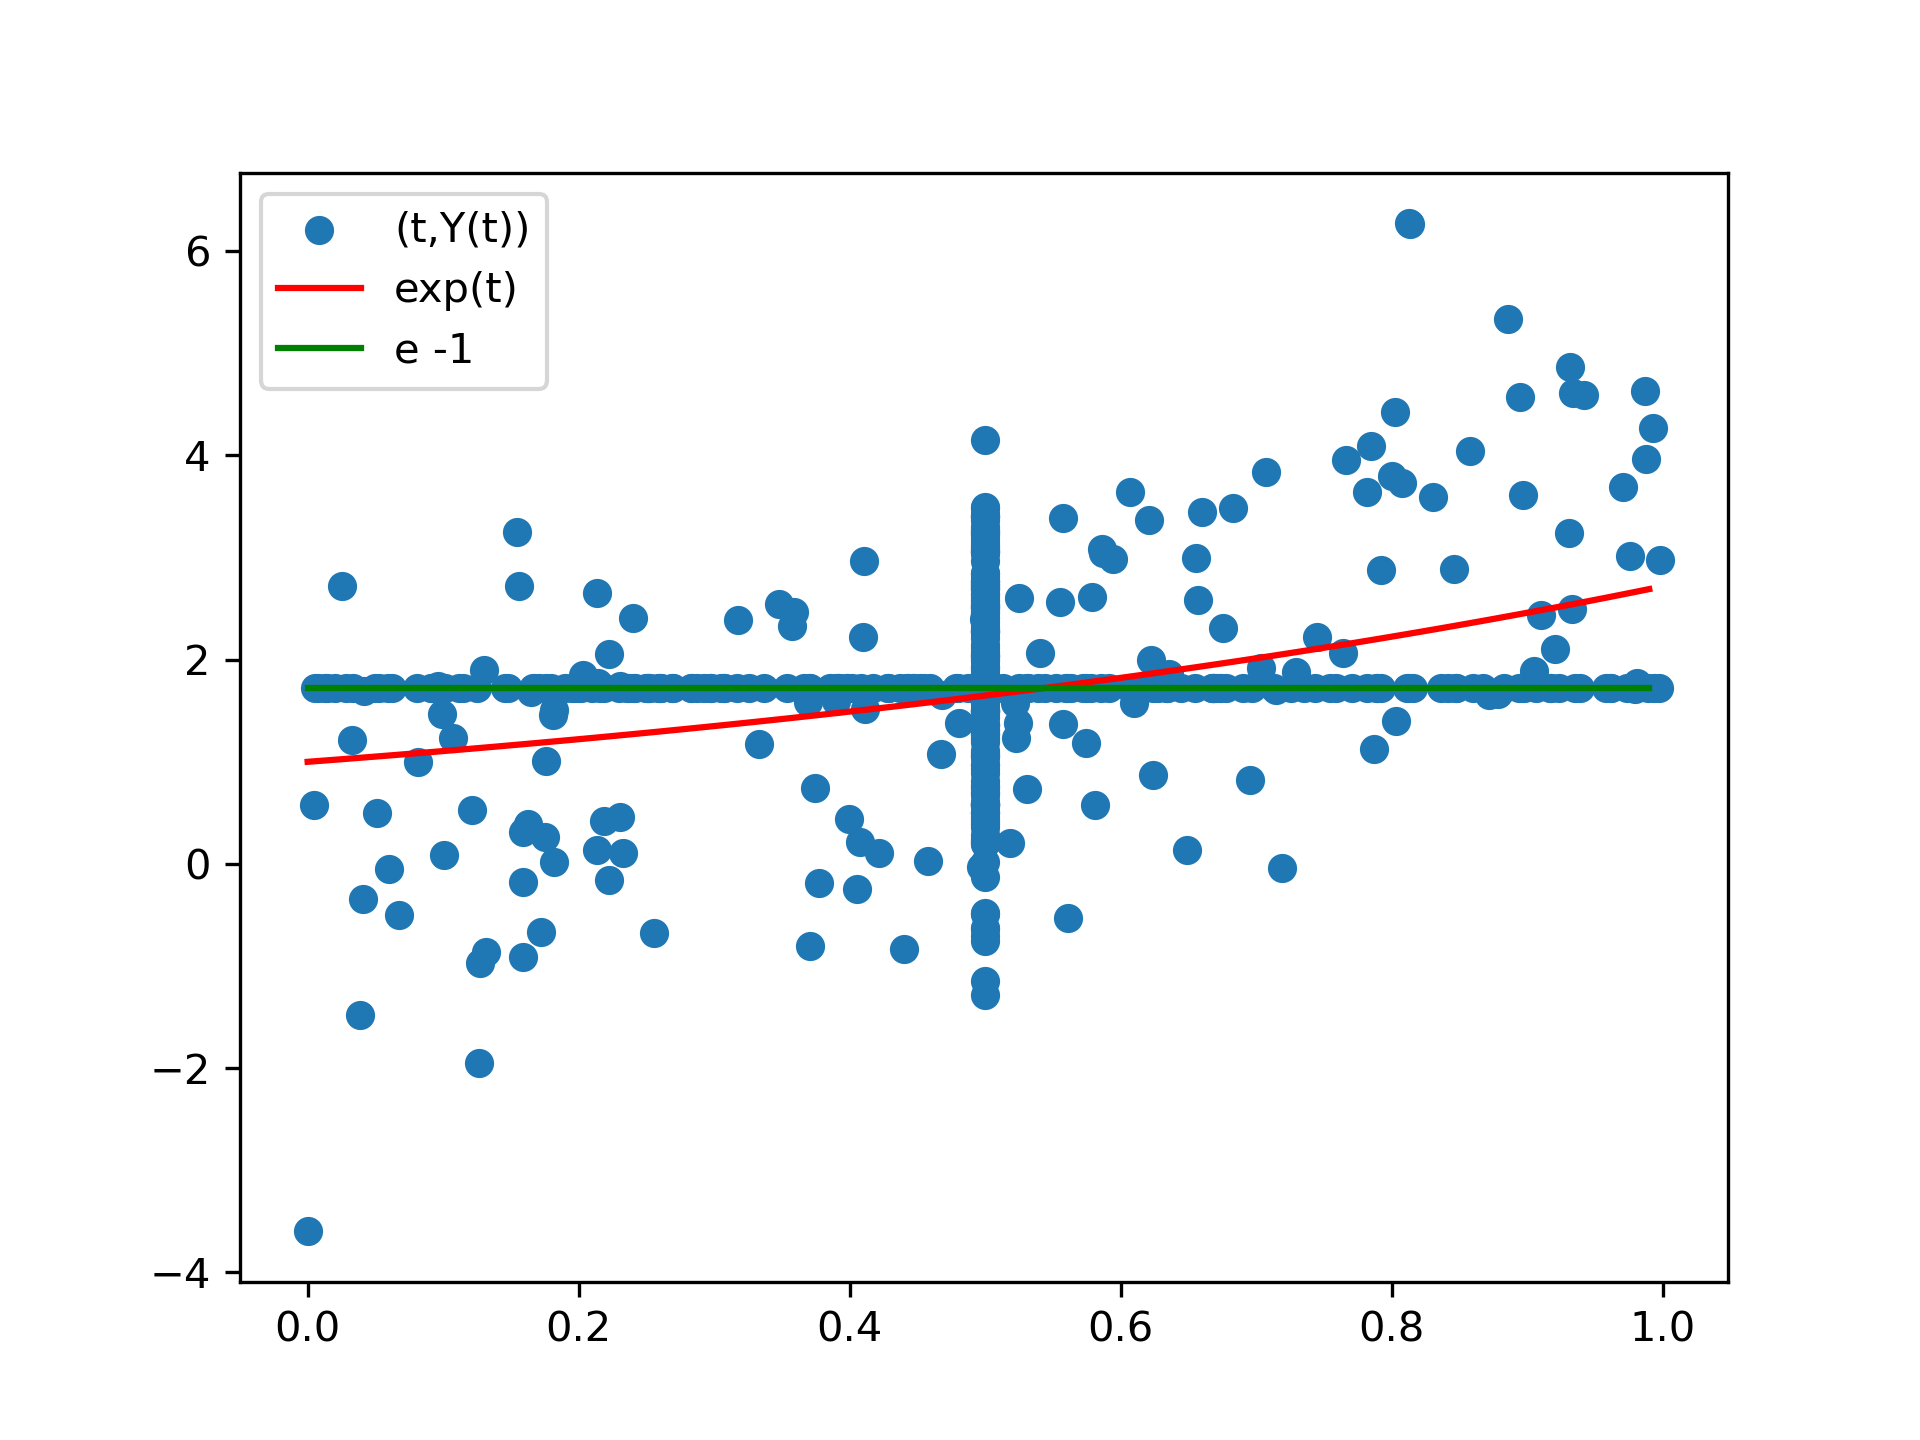
\includegraphics[width=0.8\textwidth]{plots/ydy int.png}
        \caption{Recursive calls of (\ref{RRVE ydy int}) when
            calling $Y(0.5)$ $300$ times. Points accumulate on
            the green line due to the Russian roulette,
            and at  $t=0.5$ because it is the starting
            value of the simulation.
        }
        \label{fig:ydy int}
    \end{figure}

\end{example}

\begin{example}[$y''=y$ mixed boundary conditions]
    Consider the following ODE:
    \begin{equation} \label{ddyy}
        y'' = y, \quad y(0) = 1, \quad y'(1) = e.
    \end{equation}
    This equation has the solution $y(t) = e^{t}$.
    We define the source green function $G(t,x)$ for $y''$
    and Dirichlet/Neumann boundary conditions as follows:

    \begin{equation}
        G'' = \delta(t-x), \quad G(0) = 0, \quad G'(1) = 0.
    \end{equation}

    Solving this equation yields:

    \begin{equation}
        G(t,x) =
        \begin{cases}
            -t & \text{if } t < x   \\
            -x & \text{if } t \ge x
        \end{cases}.
    \end{equation}

    We define the boundary green function $P(t,x)$
    (for $x \in {0,1}$) for $y''$ and Dirichlet/Neumann
    boundary conditions as follows:
    \begin{equation}
        P'' = 0, \quad \left(P(0,x),P'(1,x) \right) =
        \begin{cases}
            (1 , 0) & \text{ if } x=0 \\
            (0 , 1) & \text{ if } x=1
        \end{cases}.
    \end{equation}

    These are a basis for the homogeneous solutions.
    $P(t,x)$ can be solved from its definition:

    \begin{equation}
        P(t,x) =
        \begin{cases}
            1 & \text{ if } x=0 \\
            t & \text{ if } x=1
        \end{cases}.
    \end{equation}

    At this point, it may not be clear, but with this set of green functions,
    we can form the following integral equation for (\ref{ddyy}):
    \begin{equation} \label{int ddyy}
        y(t) = P(t,0)y(0) + P(t,1)y(1) + \int_{0}^{1}G(t,s) y(s) ds.
    \end{equation}

    Equation (\ref{int ddyy}) can be expressed as:
    \begin{equation} \label{RRVE ddyy}
        Y(t) = 1 + te + l B\left(\frac{1}{l}\right)G(t,S)Y(S),
    \end{equation}
    where $S \sim U$ and $l>1 \in \mathbb{R}$. We visualize
    equation (\ref{RRVE ddyy}) in Figure \ref{fig:ddyy}.

    \begin{figure}[h!]
        \centering
        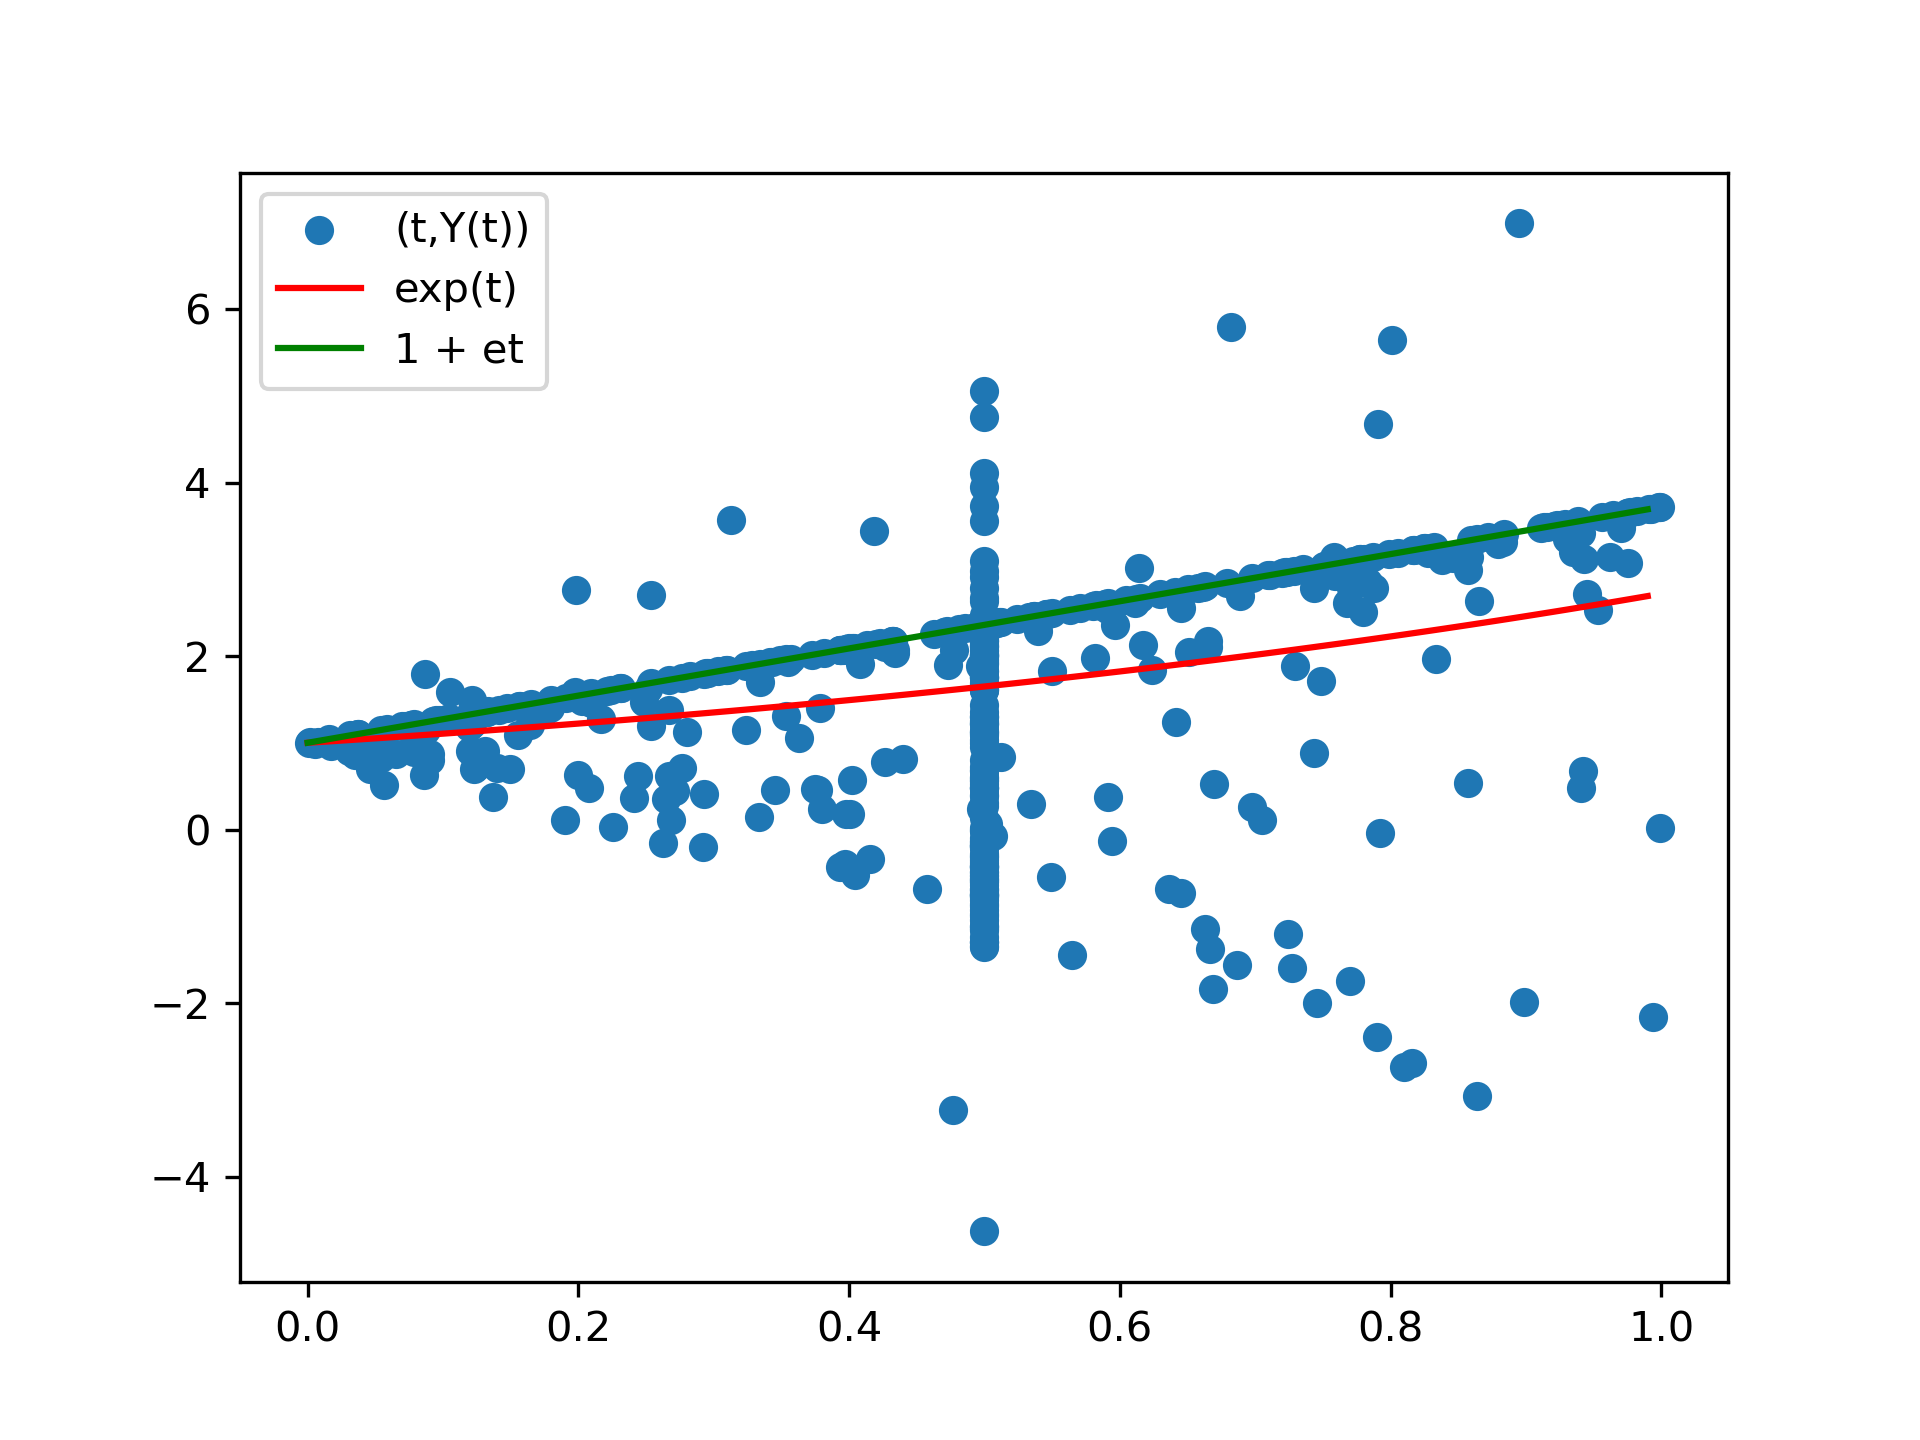
\includegraphics[width=0.8\textwidth]{plots/ddyy.png}
        \caption{Recursive calls of (\ref{RRVE ddyy}), $l=2$ when
            calling $Y(0.5)$ $300$ times.}
        \label{fig:ddyy}
    \end{figure}

\end{example}

\begin{related}[$y''=y$ mixed boundary conditions]
    \cite{sawhney_walk_2023} discusses an algorithm for mixed boundary conditions.
\end{related}


%\begin{definition}[boundary green function]
%    we write this later
%    %   The boundary green function of a linear differential problem with linear boundary
%    %   conditions.
%\end{definition}
%
%\begin{definition}[source green function]
%    we write this later
%    %    For
%    %    \[
%    %        L(y(z)) = f
%    %        .\]
%    %    with $L$ a linear differential operator, $z$ a point in the input space of $y$
%    %    ,$f$ arbitrary and linear boundary conditions.
%    %    We define the source green function $G(z,s)$ with following property
%    %    \[
%    %        L(G(z,s))=\delta(z-s).
%    %        .\C
%    %    and null boundary conditions.
%\end{definition}
%
%
%\begin{example}[numerical green functions]
%    There will be probably some green functions that we need
%    that don't have an analytic expression yet.
%\end{example}

% Green's function vs green function (check chatgpt for the answer)
\begin{definition}[green function]
    Vaguely speaking, we define the green function as a type
    of kernel function used to solve linear problems with linear
    conditions. The green function is the kernel that we
    place in front of the linear conditions or the source term,
    which we integrate over to obtain the solution. The green
    function possesses the property of satisfying either null
    linear conditions and a Dirac delta source term, or vice versa.
\end{definition}

\begin{related}[green function]
    Our notion of green function is similar to that in \cite{hwang_simulationtabulation_2001}.
\end{related}

% maybe an example of difference equation

% \subsection{Convergence}
\subsection{Fredholm Integral Equations}

\textcolor{darkgreen}{
    More related work to coupled splitting is \cite{bakbouk_mean_2023}.
    Maybe we should add some experiments where we demonstrate the 2 ways
    of converging with coupled splitting.
} \\

The integral equations obtained in the previous subsection are Fredholm integral
equations of the second kind. In this subsection, we introduce a technique called
coupled splitting.


\begin{definition}[Fredholm equation of the second kind]
    A Fredholm equation of the second kind for $\varphi$  is of the following form:
    \begin{equation}
        \varphi(t)=f(t)+\lambda \int_a^b K(t, s) \varphi(s) ds.
    \end{equation}
    Given the kernel  $K(t, s)$  and  $ f(t)$.
\end{definition}

If both $K$ and $f$ satisfy certain regularity conditions, then for sufficiently
small $\lambda$, it is relatively straightforward to establish the existence
and uniqueness of solutions using a fixed-point argument.

% We would like to have MC algorithm that converges in that case. Our best guess is
% a combination of splitting and coupling.

\begin{example}[Dirichlet $y''=y$] \label{main dirichlet}
    The following ODE will be the main testing example for
    boundary value problems:
    \begin{equation} \label{eq:main dirichlet}
        y''=y, \quad y(b_{0}),y(b_{1}).
    \end{equation}
    The green functions corresponding to $y''$ and Dirichlet conditions are:

    \begin{align}
        P(t,x) & = \begin{cases}
                       \frac{b_{1}-t}{b_{1}-b_{0}} & \text{if } x = b_{0} \\
                       \frac{t-b_{0}}{b_{1}-b_{0}} & \text{if } x = b_{1}
                   \end{cases},       \\
        G(t,s) & = \begin{cases}
                       -\frac{(b_{1}-t)(s-b_{0})}{b_{1}-b_{0}} & \text{if } s<t \\
                       -\frac{(b_{1}-s)(t-b_{0})}{b_{1}-b_{0}} & \text{if } t<s
                   \end{cases}.
    \end{align}
    Straight from these green functions you get the following integral equation and RRVE:
    \begin{align} \label{inteq:main dirichlet}
        y(t) & = P(t,b_{0}) y(b_{0}) + P(t,b_{1}) y(b_{1}) +
        \int_{b_{0}}^{b_{1}} G(t,s)y(s) ds,                  \\
        Y(t) & = P(t,b_{0}) y(b_{0}) + P(t,b_{1}) y(b_{1})
        + l B\left(\frac{1}{l} \right)(b_{1}-b_{0}) G(t,S)y(S) , \label{RRVE:main dirichlet}
    \end{align}
    where $l \in \mathbb{R}$ the Russian roulette rate is and
    $S \sim \text{Uniform}(b_{1},b_{0})$.

\end{example}

% comes straight from wikipedia
% \begin{definition}[Liouville–Neumann series]
%     The Liouville–Neumann series for a Fredholm equation of the second kind
%     is defined as
%     \begin{equation}
%         \phi(x)=\sum_{n=0}^{\infty} \lambda^n \phi_n(x).
%     \end{equation}

%     If the $n$th iterated kernel is defined as $n-1$ nested integrals of $n$ operators $K$,

%     $$
%         K_n(x, z)=\iint \cdots \int K\left(x, y_1\right) K\left(y_1, y_2\right)
%         \cdots K\left(y_{n-1}, z\right) d y_1 d y_2 \cdots d y_{n-1}
%     $$
%     $K_0$ may be taken to be $\delta(x-z)$.

%     then

%     $$
%         \phi_n(x)=\int K_n(x, z) f(z) d z
%     $$

%     With

%     $$
%         \phi_0(x)=f(x),
%     $$

%     so
% \end{definition}


% fix point argument is when von neumann series converges


\begin{example}[coupled splitting on (\ref{main dirichlet})] \label{ex:coupled splitting}
    In addition to normal splitting (see Definition \ref{def:splitting}),
    we can also split the domain in Equation (\ref{inteq:main dirichlet})
    as follows:

    \begin{align}\label{inteq:coupled splitting}
        y(t) & = P(t,b_{0}) y(b_{0}) + P(t,b_{1}) y(b_{1}) +
        \frac{1}{2} \int_{b_{0}}^{b_{1}} G(t,s)y(s) ds +
        \frac{1}{2} \int_{b_{0}}^{b_{1}} G(t,s)y(s) ds,                                             \\
        y(t) & = P(t,b_{0}) y(b_{0}) + P(t,b_{1}) y(b_{1}) + \label{inteq:coupled domain splitting}
        \int_{b_{0}}^{\frac{b_{1}+b_{0}}{2}} G(t,s)y(s) ds +
        \int_{\frac{b_{1}+b_{0}}{2}}^{b_{1}} G(t,s)y(s) ds.
    \end{align}

    By coupling, we can eliminate the additive branching recursion
    in the RRVEs corresponding to Equations (\ref{inteq:coupled splitting})
    and (\ref{inteq:coupled domain splitting}).
    This results in the following RRVE:

    \begin{equation} \label{RRVE:coupled splitting}
        X(t_{1},t_{2})=
        \begin{bmatrix}
            P(t_{1},b_{0}) & P(t_{1},b_{1}) \\
            P(t_{2},b_{0}) & P(t_{2},b_{1})
        \end{bmatrix}
        \begin{bmatrix}
            y(b_{0}) \\
            y(b_{1})
        \end{bmatrix}
        +
        W
        \begin{bmatrix}
            G(t_{1},S_{1}) & G(t_{1},S_{2}) \\
            G(t_{2},S_{1}) & G(t_{2},S_{2})
        \end{bmatrix}
        X(S_{1},S_{2}),
    \end{equation}
    where $W$ the right weighting matrix is
    (see code (\ref{py:coupled splitting})),
    and $S_{1}$ and $S_{2}$ can be chosen
    in various ways.
\end{example}

\begin{pythonn}[implementation of (\ref{RRVE:coupled splitting})] \label{py:coupled splitting}
    We implemented equation (\ref{RRVE:coupled splitting}) in example
    (\ref{ex:coupled splitting}) with recursion but in this case, it
    is also possible to implement it forwardly. \\
    \pythoncode{python code/coupled_splitting.py}

    % can probably make a better plot then this one
    \begin{figure}[h!]
        \centering
        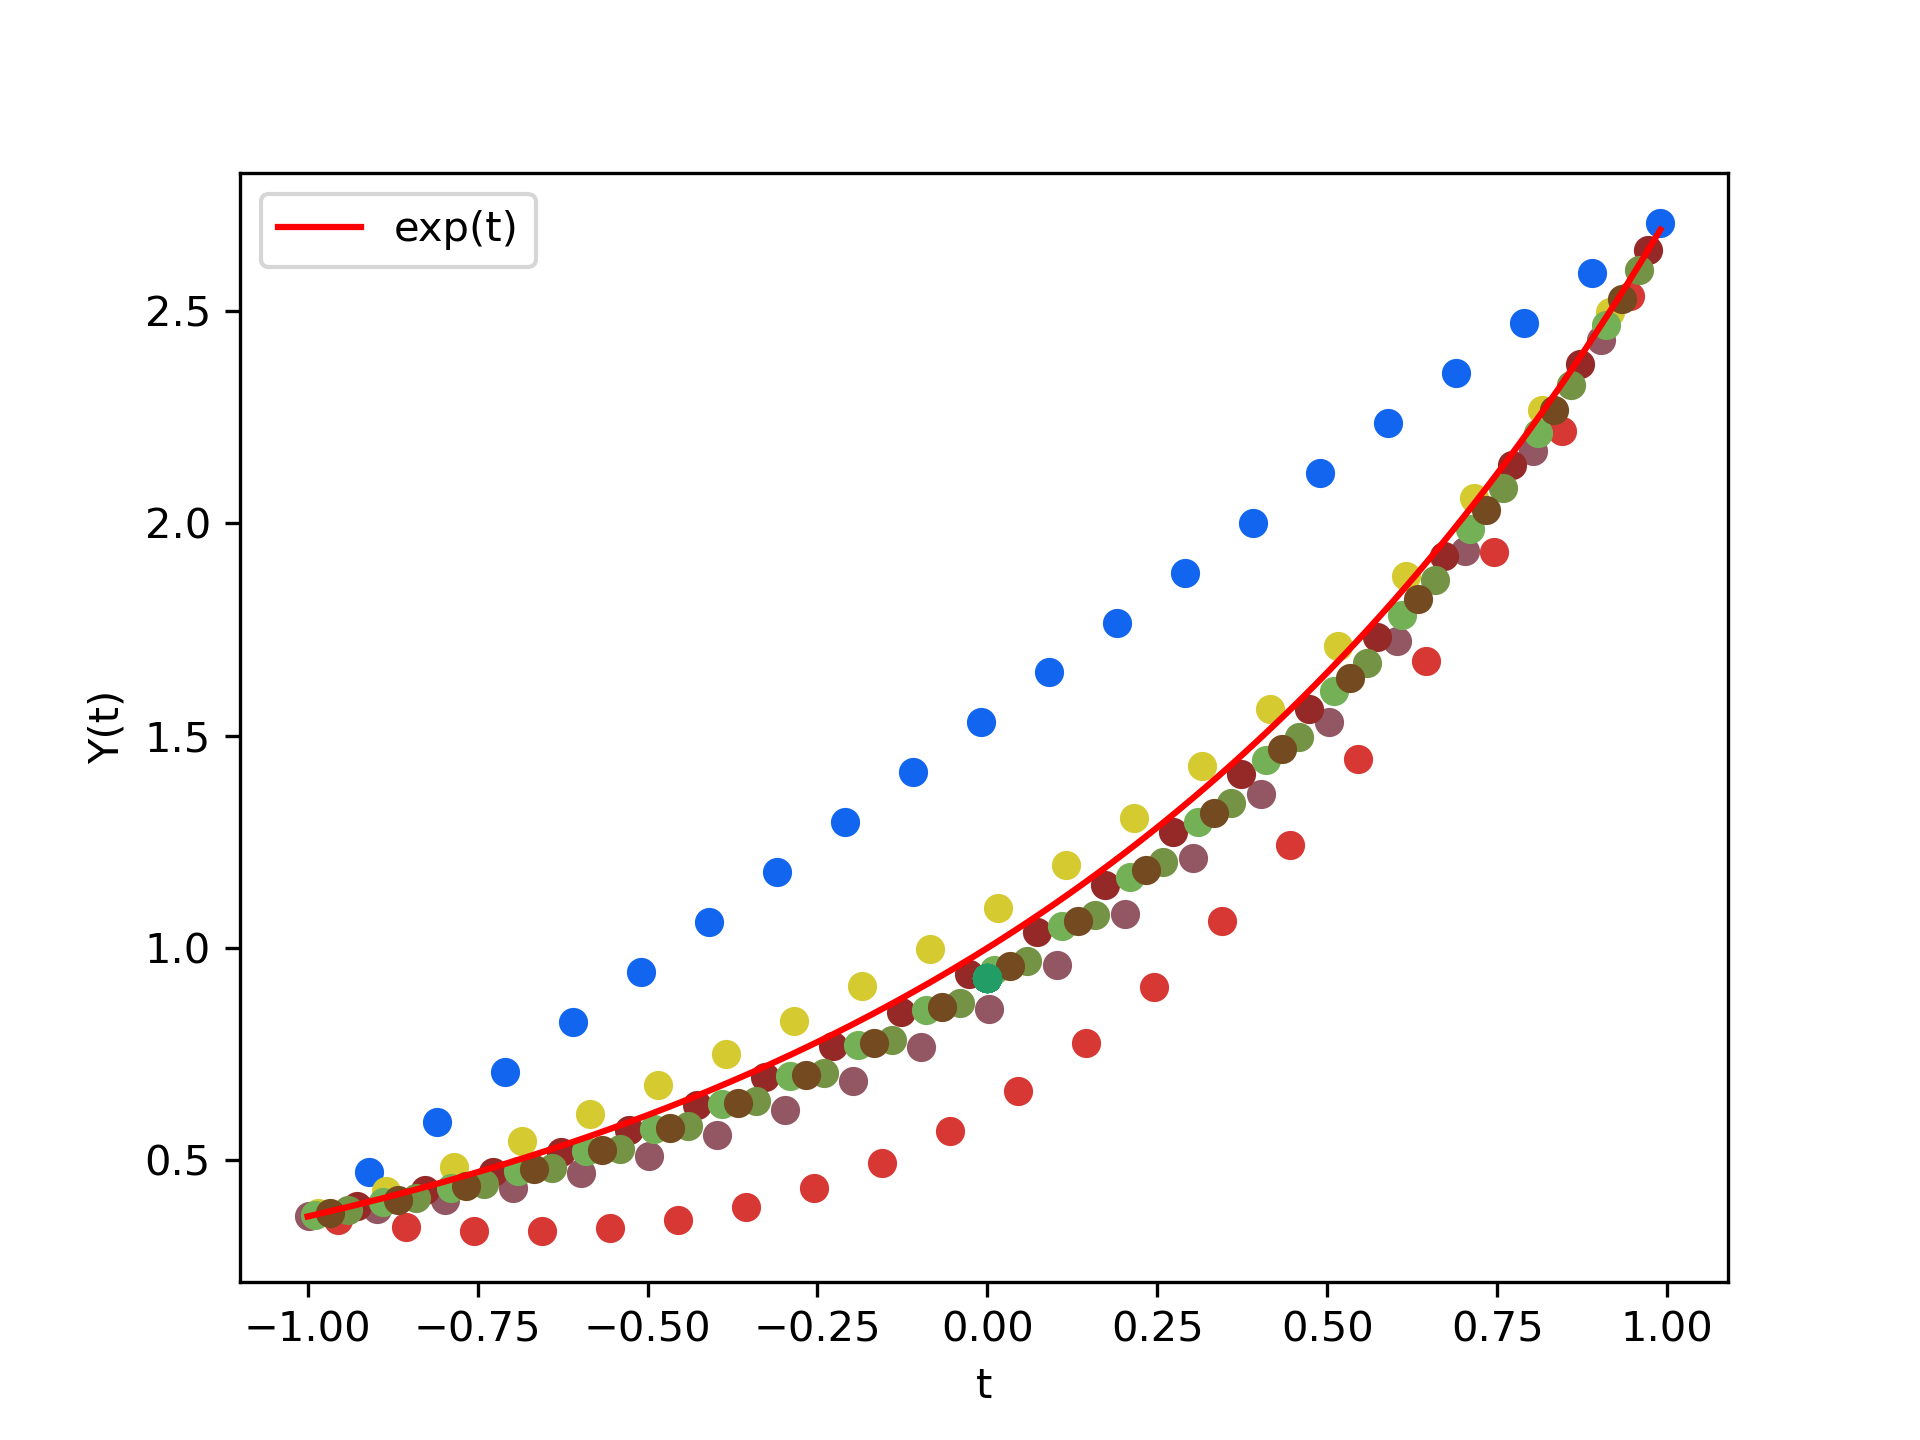
\includegraphics[width=0.8\textwidth]{plots/coupled split.png}
        \caption{Recursive calls of equation (\ref{RRVE:coupled splitting}) when
        calling $X(0)$ once,
        with a split size of $20$, $S_{j}$ are coupled such
        they are equally spaced and the coupling is colored.
        The initial conditions for this call are $y(-1)=e^{-1}$ and $y(1)=e^{1}$,
        with Russian roulette rate $l=1.2$.  }
        \label{fig:coupled splitting}
    \end{figure}
\end{pythonn}


Example (\ref{ex:coupled splitting}) does not
exploit the locality and smoothness of the problem.
We conjecture that coupled splitting can be particularly valuable when
dealing with linear Fredholm equations of the second kind,
especially in scenarios where MC integration surpasses
traditional integration methods. This holds true for
high-dimensional problems, non-smooth kernels, and
challenging domains. We conjecture that employing
coupled splitting in such cases can yield favorable results.

\begin{related}[coupled splitting]
    Coupled splitting is partly inspired by how \cite{sabelfeld_sparsified_2009}
    reduces variance by using bigger submatrices.
    Coupled splitting does not work for walk on sphere because
    of the dynamically changing domain. A technique based on reusing samples
    such as coupled splitting for walk on sphere gets discussed
    in \cite{miller_boundary_2023}.
\end{related}

% explaining that coupled split is cool for global problems but for
% ODEs and PDEs we are interested in exploiting locality.

\subsection{Initial Value Problems}

\textcolor{darkgreen}{
    We should add more metrics and
    discuss some trade-offs.
    We didn't really specify a full algorithm for any linear ODE.
    Each of our examples requires some derivation. We didn't want to commit
    to an algorithm because the choices that we made were arbitrary
    and not natural just the bare minimum to get the right behavior.
    'One does not simply implement a research idea.'
} \\


Classic IVP solvers rely on shrinking the time steps for
convergence. In this subsection we build up to
Recursion in Recursion MC (RRMC) for IVPs that tries to emulate
this behavior.


\begin{example}[RRMC $y'=y$] \label{ex:RRMC IVP}
    We demonstrate RRMC for IVPs with

    \begin{equation}
        y' = y, \quad y(0) = 1.
    \end{equation}

    Imagine we have a time-stepping scheme $(t_{n}), \forall n: t_{n-1} < t_{n}$
    then the following integral equations hold:

    \begin{equation}
        y(t)= y(t_{n}) + \int_{t_{n}}^{t}y(s)ds , \quad t>t_{n}.
    \end{equation}

    Turn these in the following class of RRVEs:

    \begin{equation}
        Y_{n}(t) = y(t_{n}) + (t-t_{n})Y_{n}((t-t_{n})U+t_{n}), \quad t>t_{n}.
    \end{equation}

    A problem with these RRVEs is that we do not know $y(t_{n})$.
    Instead, we can replace it with an unbiased estimate $y_{n}$
    which we keep frozen in the inner recursion:
    \begin{align}
        \label{eq:RRMC IVP inner}
        Y_{n}(t) & = y_{n} + (t-t_{n})Y_{n}((t-t_{n})U+t_{n}), \quad t>t_{n} \\
        y_{n}    & = \begin{cases}
                         Y_{n-1}(t_{n}) & \text{ if } n \neq 0 \\
                         y(t_{0})       & \text{ if } n = 0
                     \end{cases}.
        \label{eq:RRMC IVP outer}
    \end{align}
    We refer to equation (\ref{eq:RRMC IVP inner}) as the inner recursion and
    equation (\ref{eq:RRMC IVP outer}) as the outer recursion of the recursion in
    recursion.
\end{example}
% maybe measurements of amount of calls to f

\begin{pythonn}[implementation of (\ref{ex:RRMC IVP})] \label{py:RRMC IVP}
    \pythoncode{python code/RRMC_IVP.py}

    \begin{figure}[h!]
        \centering
        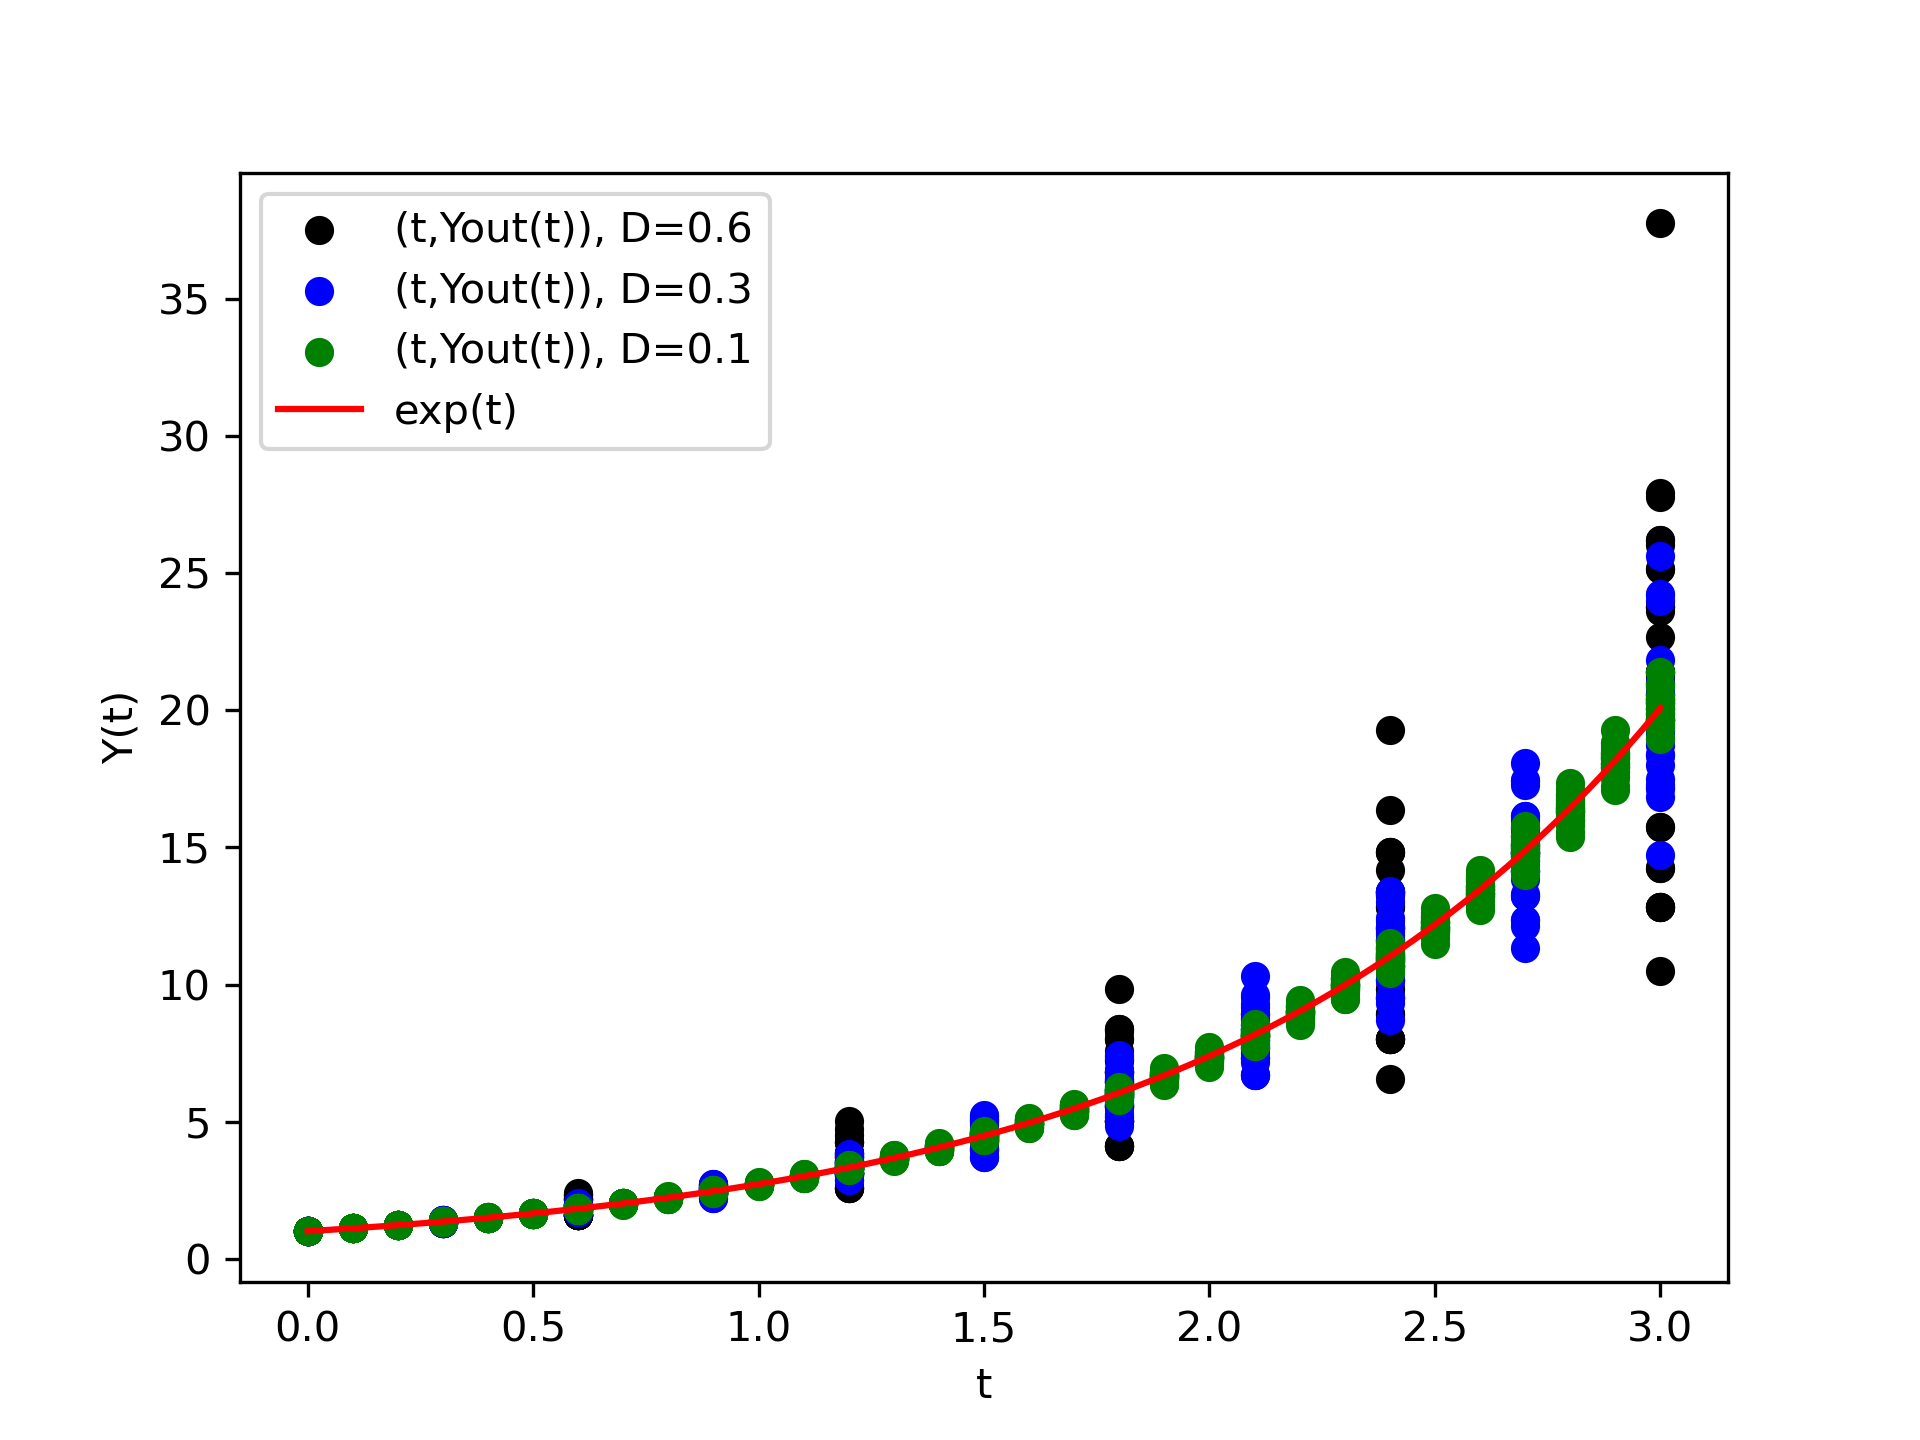
\includegraphics[width=0.8\textwidth]{plots/RRMC IVP.png}
        \caption{Recursive calls of equation (\ref{eq:RRMC IVP outer})
            when calling $Y_{\text{out}}(3,h)$ $30$ times for different $h$.  }
        \label{fig:RRMC IVP}
    \end{figure}
\end{pythonn}

We measured the convergence speed of example (\ref{ex:RRMC IVP}) to
be $O\left(\frac{h^{1.5}}{\sqrt{\text{nsim}}} \right)$.
While a $1.5$ order of convergence is commendable for an unbiased method,
it raises the question of how to attain even higher convergence orders.
It is possible to emulate classical methods to
achieve a higher order of convergence. This can be accomplished by eliminating
lower order terms by using control variates, as demonstrated in the MC trapezoidal
rule (see \ref{MCtrap}).

\begin{example}[CV RRMC $y'=y$]\label{ex:CV RRMC IVP}
    Let us control variate example (\ref{ex:RRMC IVP}).

    \begin{equation}
        y(t)= y(t_{n}) + \int_{t_{n}}^{t}y(s)ds , \quad t>t_{n}.
    \end{equation}

    We build a control variate with a lower-order approximation
    of the integrand:

    \begin{align}
        y(s) & = y(t_{n}) + (s-t_{n})y'(t_{n}) + O((s-t_{n})^{2})       \\
             & \approx y(t_{n}) + (s-t_{n})f(y(t_{n}),t_{n})            \\
             & \approx y(t_{n}) +
        (s-t_{n})\left(\frac{y(t_{n})-y(t_{n-1})}{t_{n}-t_{n-1}}\right) \\
             & \approx y(t_{n})(1+s-t_{n}).
    \end{align}

    Using the last one as a control variate for the integral:

    \begin{align}
        y(t) & = y(t_{n}) + \int_{t_{n}}^{t}y(s)ds                                          \\
             & = y(t_{n}) + \int_{t_{n}}^{t}y(s)-y(t_{n})(1+s-t_{n}) +y(t_{n})(1+s-t_{n})ds \\
             & = y(t_{n})\left(1 + (1-t_{n})(t-t_{n})+\frac{t^{2}-t_{n}^{2}}{2}\right)
        + \int_{t_{n}}^{t}y(s)-y(t_{n})(1+s-t_{n})ds.
    \end{align}

    We will not discuss turning this into an RRVE nor the implementation.
    The implementation is very similar to (\ref{py:nonlinear RRMC IVP}) and
    Figure \ref{fig:CV RRMC IVP} is a convergence plot for this example.

    \begin{figure}[h!]
        \centering
        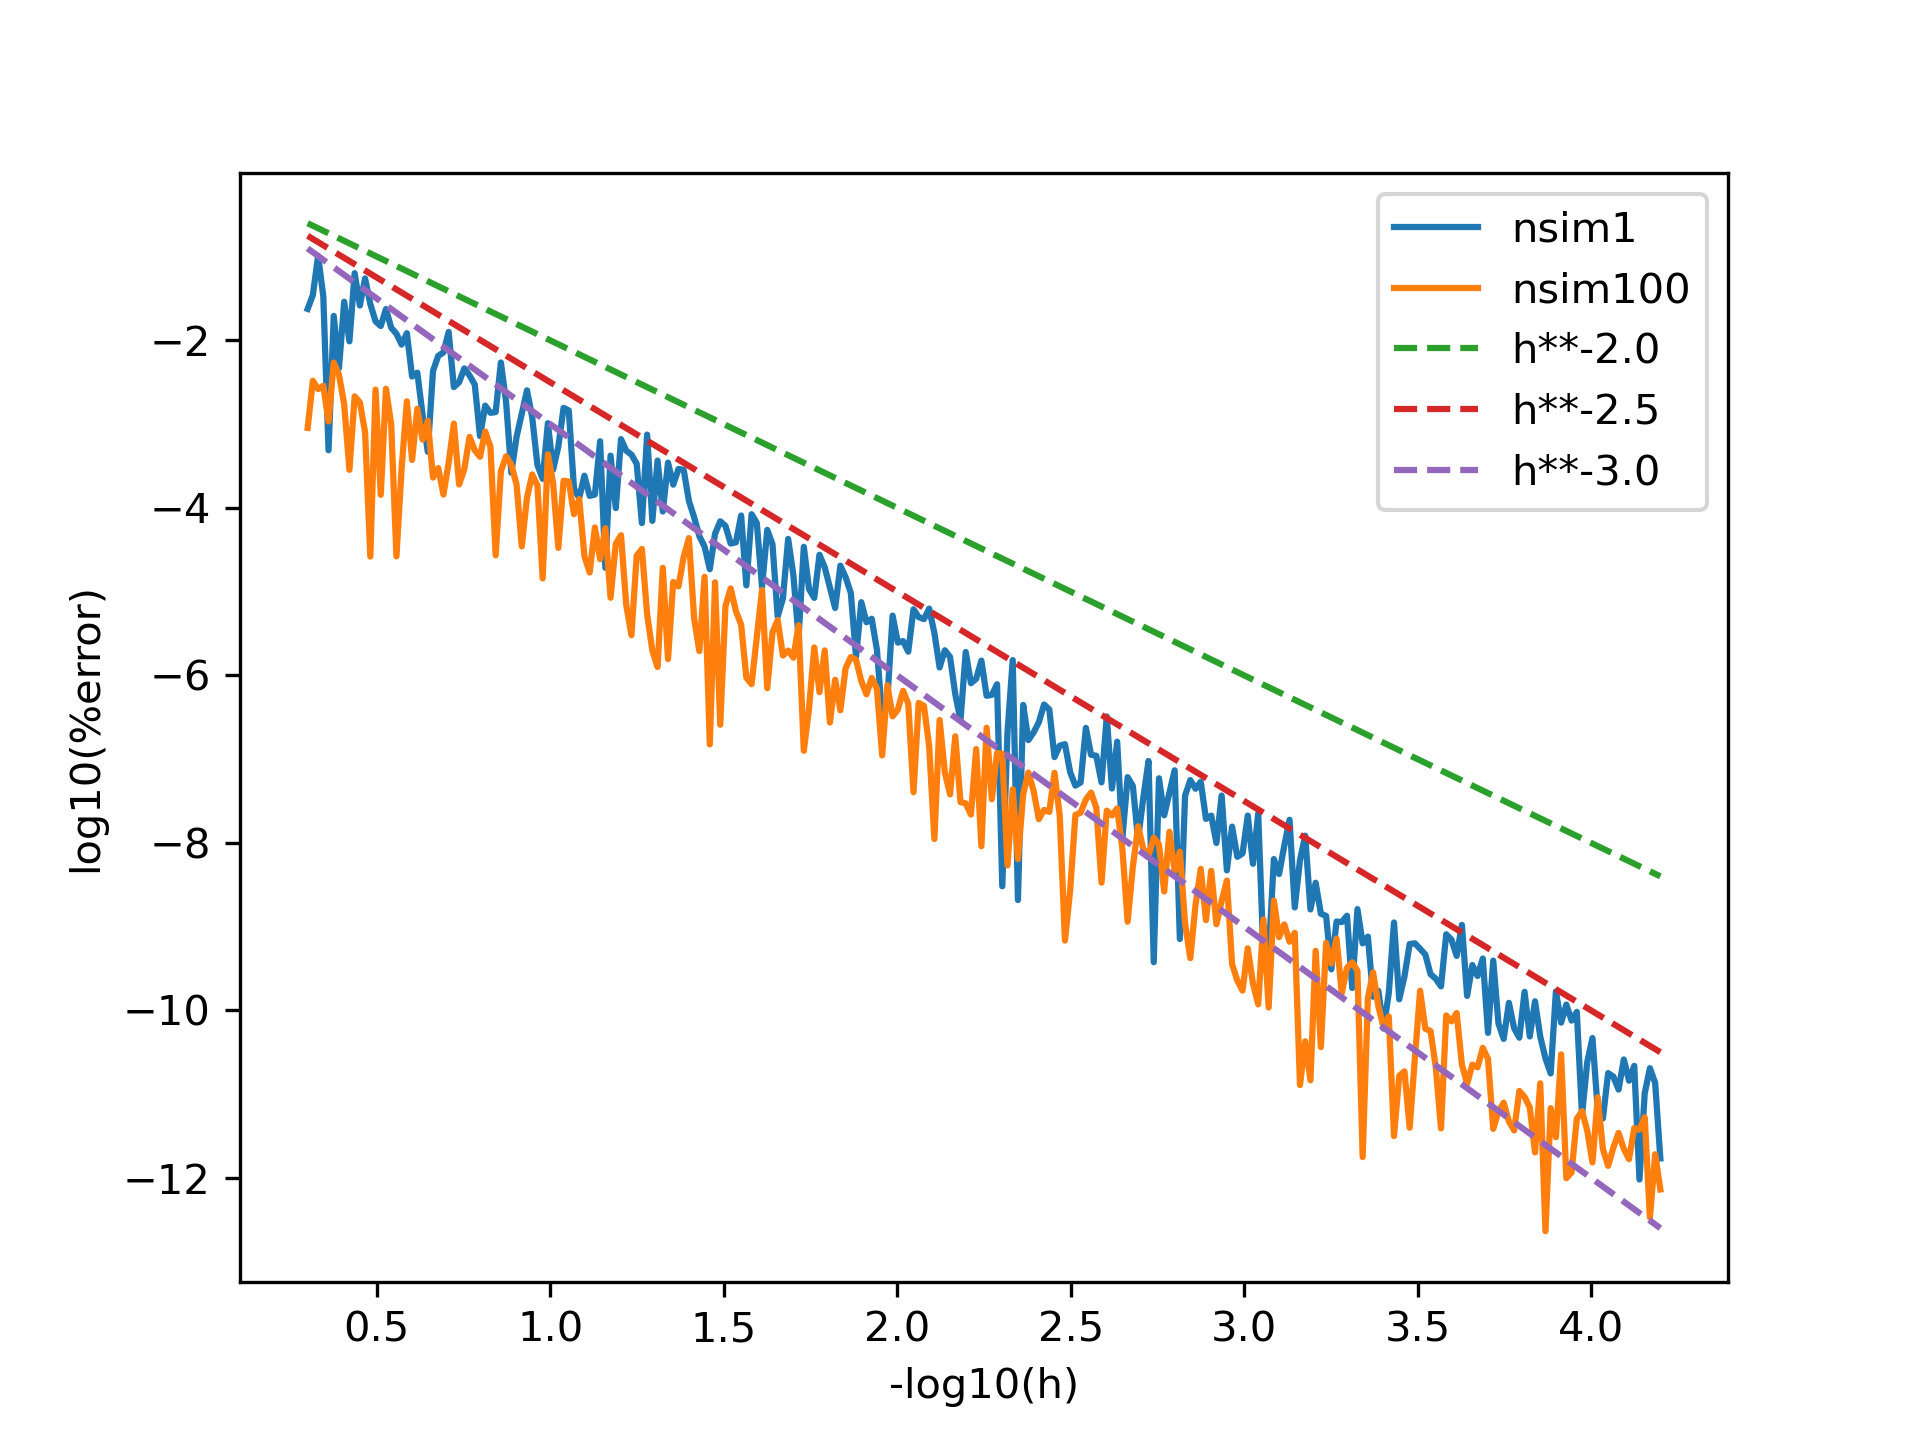
\includegraphics[width=0.8\textwidth]{plots/CV RRMC IVP.png}
        \caption{Log-log plot of the error for example
            (\ref{ex:CV RRMC IVP}) at $Y(10)$.}
        \label{fig:CV RRMC IVP}
    \end{figure}
\end{example}

\begin{related}[CV RRMC]
    \cite{daun_randomized_2011} similarly uses control variates to achieve
    a higher order of convergence.
\end{related}

RRMC is biased for our approach to non-linear problems.
The inner recursions are correlated because they use the same
information from the outer recursions, this does not mean that reducing
root-mean-square error by splitting does not work, you just have to be careful
with the bias. We conjecture that the bias in RRMC converges faster than the
variance when decreasing $h$.


\begin{example}[nonlinear RRMC IVP] \label{ex:nonlinear RRMC IVP}
    Consider the following IVP:

    \begin{equation}
        y' = y^{2} - t^{4} + 2t, \quad y(0) = 0.
    \end{equation}

    The exact solution to this problem is given by $y(t) = t^{2}$.
    We can express the solution as an integral equation:

    \begin{equation}
        y(t) = y(t_{n}) + \int_{t_{n}}^{t} y^{2}(s) ds
        - \frac{t^{5}-t_{n}^{5}}{5} + (t^{2}-t_{n}^{2}).
    \end{equation}

    By control variating $y^2(s)$ up to the second order using Taylor expansion,
    we have:

    \begin{align}
        y^2(t) & \approx y^2(t_n) + 2(t-t_n)y(t_n)y'(t_n) + ((t-t_n)y'(t_n))^2 + O((t-t_n)^2) \\
               & \approx y^2(t_n) + 2(t-t_n)y(t_n)y'(t_n) + O((t-t_n)^2)
    \end{align}

    Integrating the control variate yields:

    \begin{align}
        \int_{t_{n}}^{t} & y^{2}(t_{n}) + 2(s-t_{n})y(t_{n})y'(t_{n}) ds \\
                         & = (t-t_{n})y^{2}(t_{n})+
        2\left(\frac{t^{2}-t_{n}^{2}}{2} -t_{n}(t-t_{n}) \right)y(t_{n})y'(t_{n}).
    \end{align}
    We implement this example in (\ref{py:nonlinear RRMC IVP}).
\end{example}

\begin{pythonn}[implementation of (\ref{ex:nonlinear RRMC IVP})] \label{py:nonlinear RRMC IVP}
    \pythoncode{python code/nonlinear_CVRRMC.py}
\end{pythonn}


% \subsection{BVPs ODEs}

% Now we hope we can imitate what we did for IVPs to get converging RMC
% algorithms for BVPs. The $2$ essential trick that we used for RRMC IVP are
% integral representations on subdomains and unbiased estimators for the linear
% conditions. \\

% TODO: fix it or leave it out
% \begin{example}[alternating RRMC]
%     We demonstrate alternating RRMC on example (\ref{main dirichlet})
%     with $y(-2)=e^{-2}$ and $y(2)=e^{2}$ which didn't have convergence on
%     (\ref{fig:mainD explosion}).
%     In alternating RRMC we use integral equations of overlapping domains see Figure
%     (\ref{fig:alternating RRMC}) and communicate boundary conditions in the outer recursion.
%     \begin{figure}[h!]
%         \centering
%         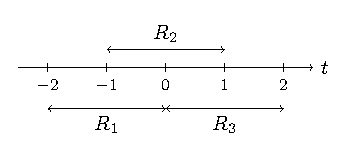
\includegraphics[width=0.8\textwidth]{tikz figures/local RRMC/axis.pdf}
%         \caption{}
%         \label{fig:alternating RRMC}
%     \end{figure}
% \end{example}

% \begin{related}
%     Schwarz alternating method, walk on rectangles paper.
% \end{related}

\subsection{Limitations and Future Work}

\textcolor{darkgreen}{
    DRRMC is irrelevant and should be removed.
} \\

We have not dedicated significant attention, if any at all, to
the convergence analysis of RMC methods
for Fredholm equations. Figure \ref{fig:mainD explosion} illustrates
that arbitrary RMC do not converge. \\

Coupled splitting was tested on the example shown in Figure
\ref{fig:mainD explosion}, but it did not contribute to the
convergence of the method. This suggests that a fix point argument
would not be effective for this particular example with this
Russian roulette setup. \\

\begin{figure}[h!]
    \centering
    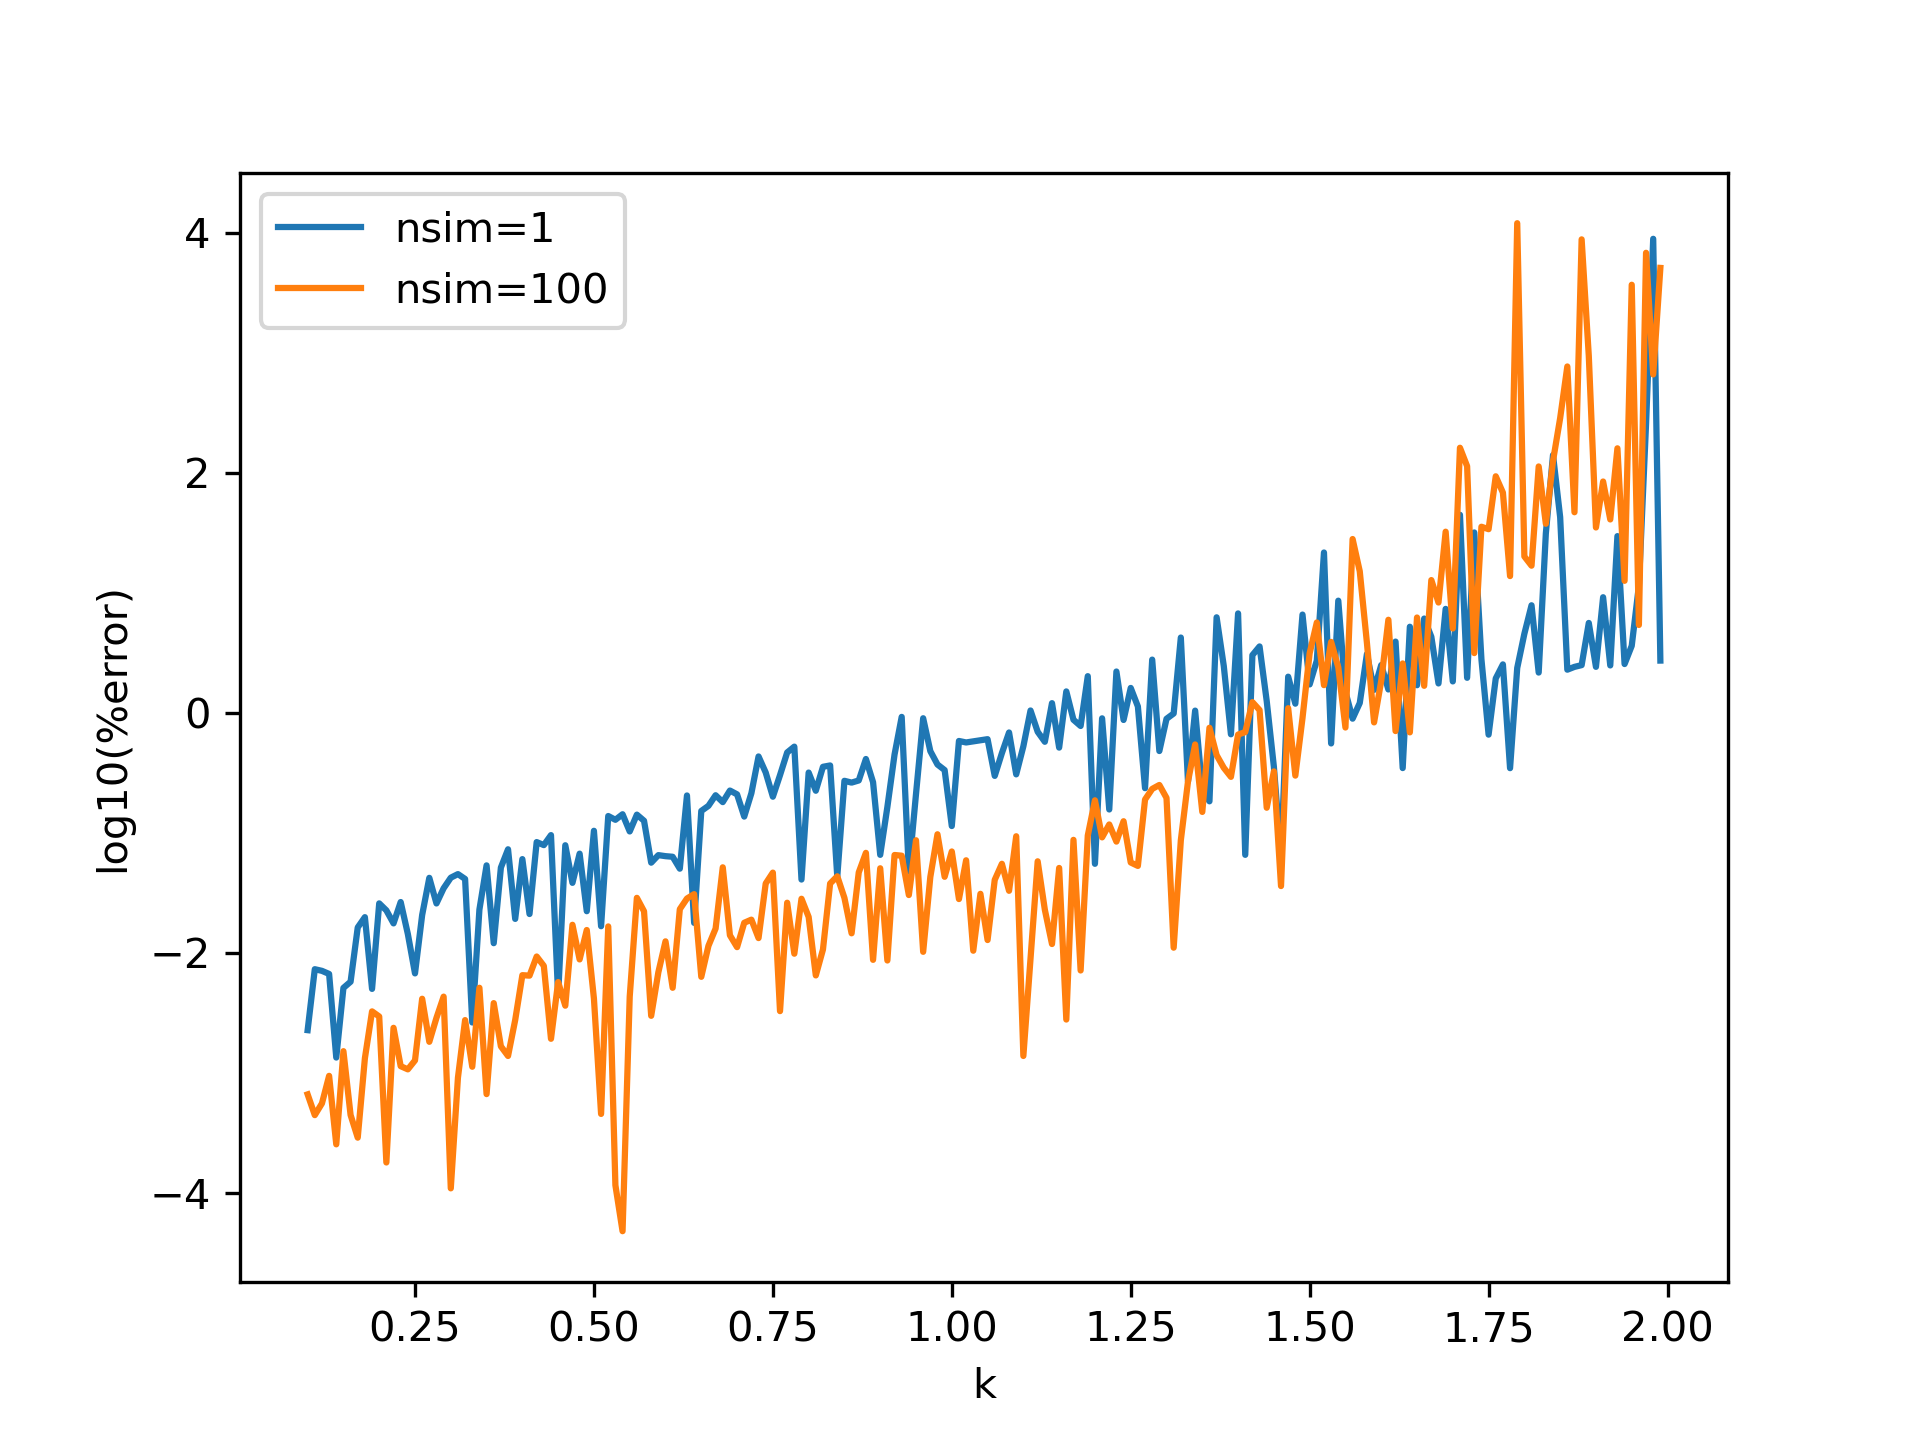
\includegraphics[width=0.8\textwidth]{plots/mainD explosion.png}
    \caption{The logarithmic percentage error of $Y(0)$ for
    (\ref{RRVE:main dirichlet}), with $l=1.2$ and initial conditions
    $y(-k)=e^{-k}$ and $y(k)=e^{k}$, displays an exponential
    increase until approximately $k=1.5$, beyond which additional
    simulations fail to reduce the error, indicating that the variance
    doesn't exist.}
    \label{fig:mainD explosion}
\end{figure}


Figure \ref{fig:coupled splitting}
resembles fixed-point iterations, leading us to hypothesize
that coupled splitting can achieve convergence in most cases
where a fixed-point argument holds true and the convergence
speed is very similar to fix-points methods until the accuracy
of the stochastic approximation of the operator is reached
(the approximate operator bottleneck). The approximation of the operator
can be improved by increasing coupled splitting amount when
approaching the bottleneck. Alternatively when reaching
the bottleneck it is possible to rely on MC convergence.

\begin{related}[convergence coupled splitting]
    See \cite{gupta_convergence_2021} for a discussion on the convergence
    of recursive stochastic algorithms. We highly recommend watching
    the corresponding video \cite{abhishek_gupta_recursive_2020} before reading
    the paper.
\end{related}

% (Additional
% iterations beyond the bottleneck do not
% bring the solution closer but they still remain unbiased with low variance)

Similarly to classic methods, RRMC struggles with big negative coefficients in front
of the recursive parts which may appear in
stiff problems. We tested DRRMC as a potential remedy but we conclude
it to be ineffective.

\begin{definition}[DRRMC]
    Consider a general linear ODE IVP problem:
    \begin{equation}
        x' = Ax+g, \quad x(0)= x_{0}.
    \end{equation}
    Sometimes repeatedly multiplying by $A$ is unstable.
    Diagonal RRMC adds a positive diagonal matrix $D$
    to $A$ and hopes that it stabilizes.

    \begin{equation}
        x' + Dx = (A+D)x+g.
    \end{equation}

    The following integral equation can be derived by using integrating factor:

    \begin{equation}\label{eq:int eq DRRMC}
        x(t)= e^{D(t_{n}-t)}x(t_{n}) + \int_{t_{n}}^{t} e^{D(s-t)}(A+D)x(s)ds+\int_{t_{n}}^{t} e^{D(s-t)}g(s)ds.
    \end{equation}

    Remember that the exponential of a diagonal matrix is the exponential of its elements.
    The recursive integral has the following trivial control variate:

    \begin{equation}\label{eq: CV DRRMC}
        \int_{t_{n}}^{t}  e^{D(s-t)}(A+D)x(t_{n})ds = D^{-1}(I-e^{D(t_{n}-t)})(A+D)x(t_{n}).
    \end{equation}

    Note that $D$ may be chosen differently for every outer recursion.
\end{definition}

\begin{example}[DRRMC] \label{ex:DRRMC}
    Consider:
    \begin{equation}
        x'= Ax, x(0)=
        \begin{bmatrix}
            1 \\
            0
        \end{bmatrix}.
    \end{equation}

    With

    \begin{equation}
        A = \begin{bmatrix}
            0     & 1     \\
            -1000 & -1001
        \end{bmatrix}.
    \end{equation}

    This has the following solution:

    \begin{equation}
        x(t) = \frac{1}{999}
        \begin{bmatrix}
            -  e^{-1000t}+ 1000 e^{-t} \\
            1000 e^{-1000t}- 1000e^{-t}
        \end{bmatrix}.
    \end{equation}

    We choose $D$ fixed over all outer recursions:

    \begin{equation}
        D = \begin{bmatrix}
            1 & 0    \\
            0 & 1000
        \end{bmatrix}.
    \end{equation}

    We make the convergence plot for this example with
    integral equation  (\ref{eq:int eq DRRMC}) with control variate
    (\ref{eq: CV DRRMC}) implemented with recursion in recursion
    on Figure \ref{fig:DRRMC}.

    \begin{figure}[h!]
        \centering
        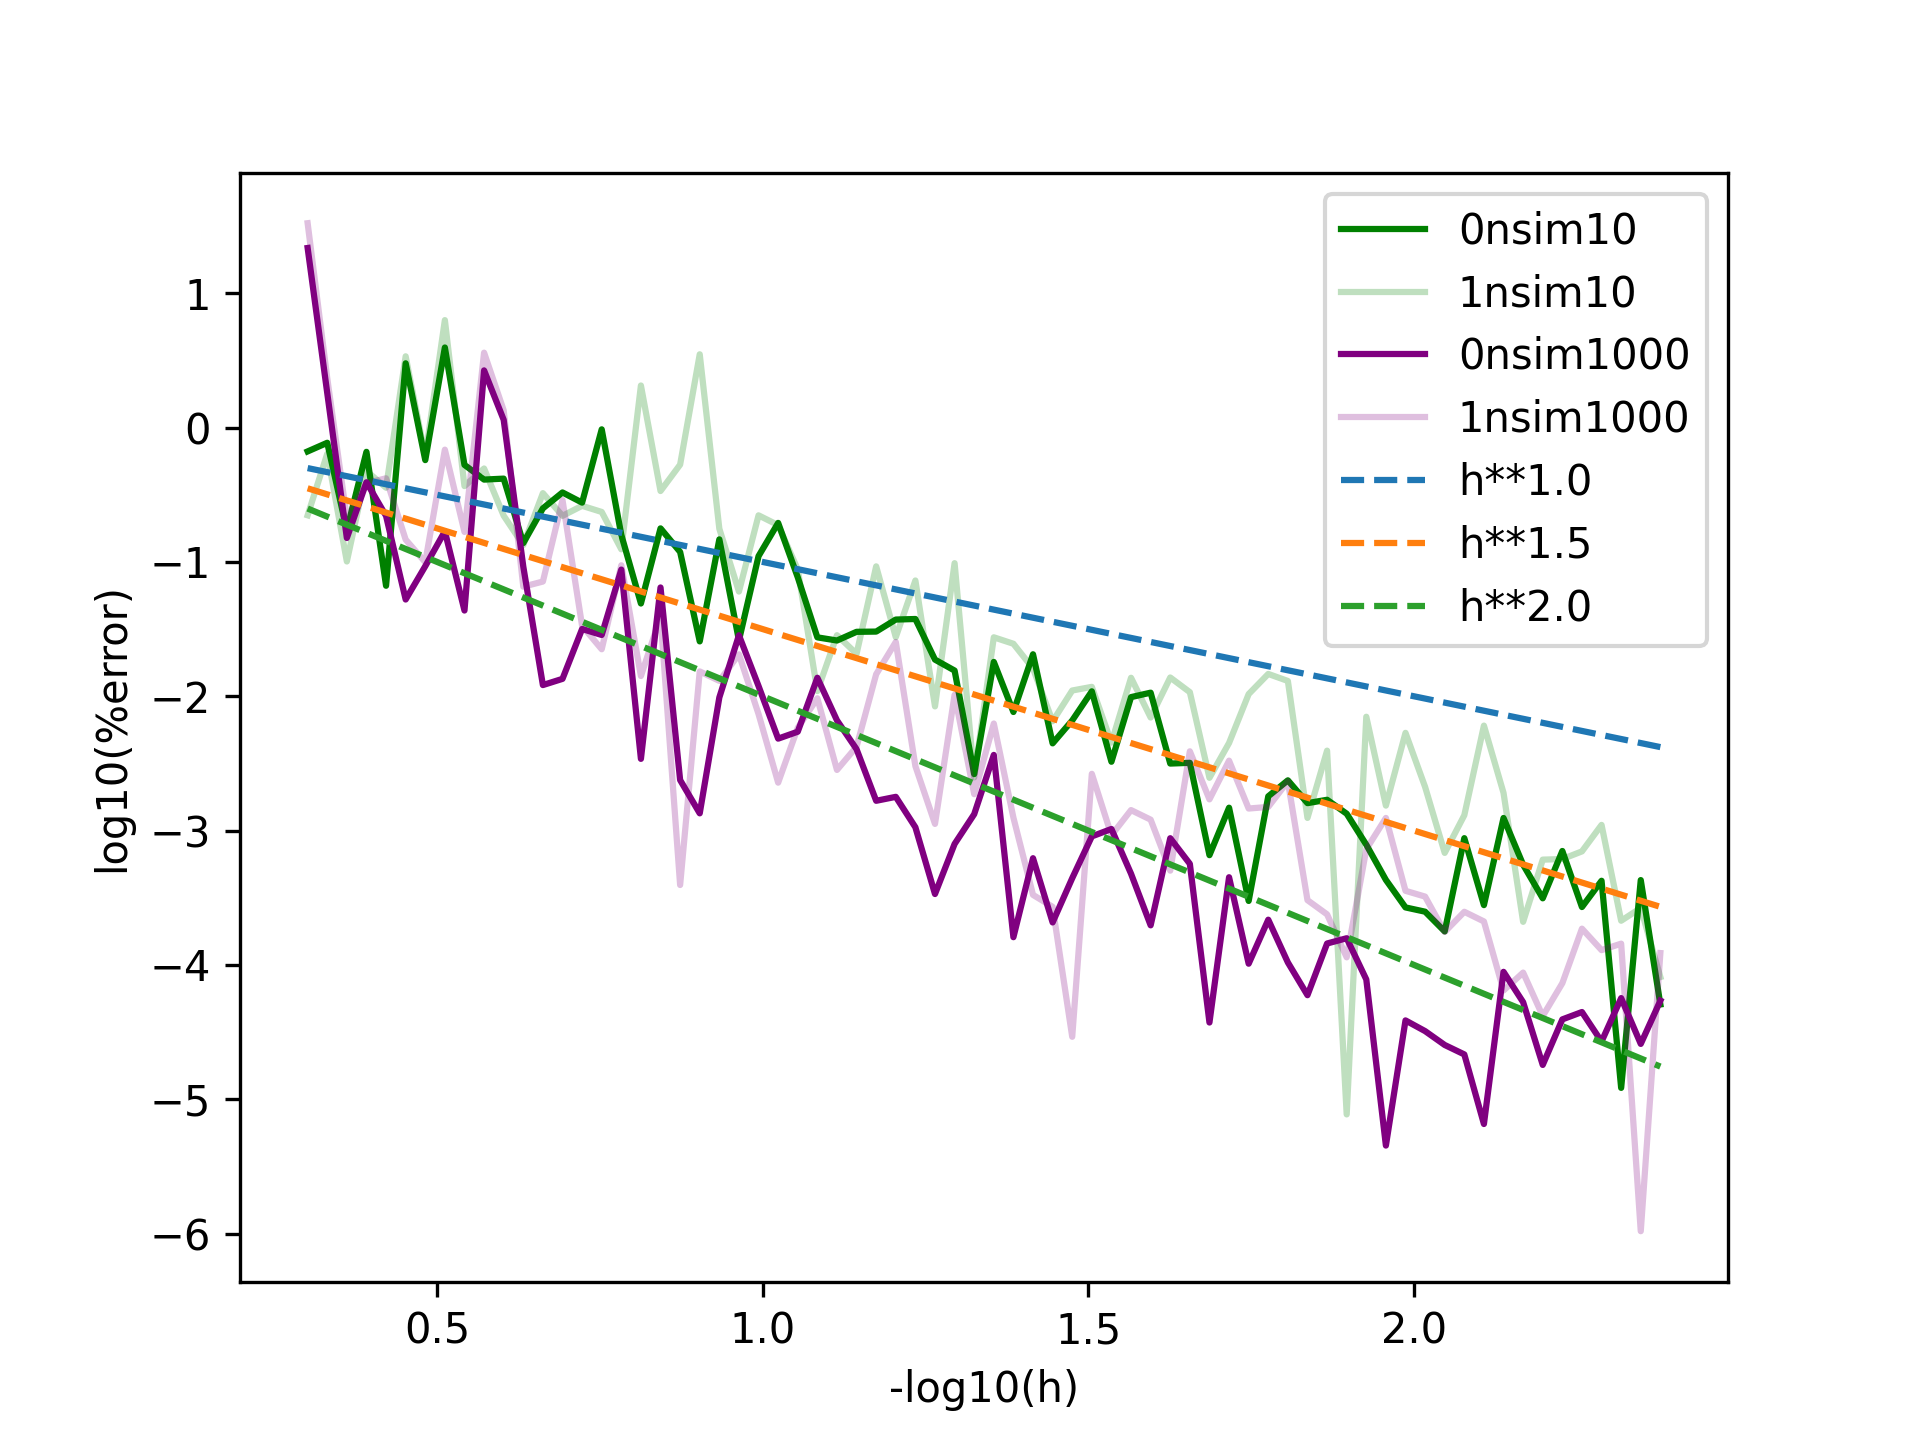
\includegraphics[width=0.8\textwidth]{plots/DRRMC.png}
        \caption{Log-log plot of the error of example (\ref{ex:DRRMC}).
            We plotted the second component of the error transparent.
        }
        \label{fig:DRRMC}
    \end{figure}

\end{example}

% TODO: 
% (critical path and how to measure performance)  see period 6 tests

\begin{related}[DRRMC]
    DRRMC is inspired by  $\bar{\sigma}$ parameter in \cite{sawhney_grid-free_2022} but
    instead of importance sampling we use control variates to deal with
    nonlinearity introduced by the exponential because it needs to work over
    an entire vector at the same time. Ideas from exponential integrator methods may
    improve DRRMC.
\end{related}

In addition to the challenges with stiff problems, we have not conducted
a comparison between RRMC and traditional methods, and we do not anticipate
that RRMC in this form outperforms other classic methods.
The reason for this is that RRMC involves
many function calls in the inner recursion without updating the current control
variate. Proper testing requires precise tuning of the MC techniques utilized.
We do believe that RRMC could potentially offer advantages in atypical scenarios.
In the following example, we examine an ODE with a random parameter.

\begin{example}[random ODEs] \label{ex:random ode}
    Consider the problem given by the initial value problem
    \begin{equation}\label{eq:random ode}
        Y' = AY, \quad Y(0)=1, \quad A \sim \text{Uniform}(0,1).
    \end{equation}
    The solution to this problem is given by
    $Y(t) = e^{tA}$, which is a RV.
    In order to compute expectations of functions of $Y(t)$,
    we use unbiased estimates $X$ of the simulations of the solution.

    Given an analytic function $f$, we can obtain $E[f(Y(t))]$
    by conditioning on the value of $A$ and using the
    law of total expectation:
    \begin{align}
        E_A[f(Y(t))] & = E_A[f(Y(t)) \mid A]         \\
                     & = E_A[f(E_X[X(t,A)]) \mid A].
    \end{align}

    To estimate $f(E_X[X(t,A)])$, we use the approach outlined in
    (\ref{ex:exp int}). For the specific example of (\ref{eq:random ode}),
    we can compute the first two moments of $Y(t)$ as
    \begin{align}
        E_A[Y(t)]   & = \frac{e^t}{t} - \frac{1}{t},      \\
        E_A[Y^2(t)] & = \frac{e^{2t}}{2t} - \frac{1}{2t}.
    \end{align}
\end{example}

\begin{pythonn}[implementation of (\ref{ex:random ode})]
    \pythoncode{python code/random_ODE.py}
\end{pythonn}


\section{Brownian Motion}

\textcolor{darkgreen}{
    We conjecture that we could use RRMC from the previous section
    to solve the heat equation and derive (discrete) next-flight walk on spheres.
} \\

Current RMC algorithms for PDEs are related to Brownian motion. In this section,
we explore the relationship between the heat equation and Brownian motion,
and discuss how recursive first-passage sampling fits into the picture.


\subsection{Heat Equation}
In this subsection, we introduce the relation between the heat equation and
Brownian motion.

% \begin{definition}[Brownian motion]
%     Define Brownian motion $W_{t}$ as the limit/logical generalization
%     when $n \rightarrow \infty$ of the following discrete process is defined as:
%     \begin{equation}
%         \begin{cases}
%             X_{t}^{n} = X_{t-\frac{1}{n}}^{n} + Z_{n} \\
%             X^{n}_{0}=0
%         \end{cases}.
%     \end{equation}
%     With $Z_{n}\sim N(0,\frac{1}{n})$ i.i.d . From this definition it is easily seen that
%     $W_{t} \sim N(0,t)$.
% \end{definition}


\begin{lemma}[self-affinity Brownian motion] \label{lem:self affine}
    Brownian motion is a self-affine random process, which implies
    that any subpath can be translated and scaled in such a way
    that its distribution matches that of the entire path.

    \begin{equation}
        \forall c \in \mathbb{R}^{+}_{0}: \frac{W_{ct}}{\sqrt{c}} \sim W_{t}.
    \end{equation}
\end{lemma}

\begin{definition}[$1$D heat equation Dirichlet] \label{def:heat equation}
    We define the $1$D heat equation for $u$ on connected domain $\Omega$
    with  Dirichlet boundary conditions the following way:
    \begin{equation}
        \frac{\partial u}{\partial t} = \frac{\partial^{2} u}{\partial x ^{2}}.
    \end{equation}
    Given $u(x,t)=\psi(x,t) ,\forall (x,t) \in \partial \Omega: t<\sup \{
        t| (x,t) \in \Omega\}$ .
\end{definition}

% maybe should improve this 
Figure \ref{fig:Euler first passage para} shows how the Dirichlet condition
is defined for parabola but reverse in time.


\begin{lemma}[Brownian motion and the heat equation] \label{lem:BM HE}
    For problem (\ref{def:heat equation}) if $ |\psi|$ is bounded
    then there holds:

    \begin{equation}
        u(x,t)=E[\psi(Y_{\tau},\tau) | Y_{t} =x].
    \end{equation}
    With $dY_{s} = dW_{-s},\tau = \sup\{s | (Y_{s},s) \notin \Omega\}$.
\end{lemma}


\begin{proof} \label{proof: BM HE }
    Discretize the heat equation
    with a regular rectangular mesh that includes $(x,t)$ with equally
    spaced intervals over space and time ($\Delta x, \Delta t$) with
    the corresponding difference equation:

    \begin{equation}
        \frac{u(x,t)-u(x,t-\Delta t)}{\Delta t} = \frac{u(x + \Delta x,t)-2 u(x,t) +u(x - \Delta x,t)}{\Delta x^{2}} .
    \end{equation}

    Isolate $u(x,t)$:

    \begin{equation} \label{eq:discrete iso heat equation}
        u(x,t) =
        \frac{\Delta t}{ 2 \Delta t + \Delta x^{2}}
        \left(
        u(x+\Delta x,t)+u(x-\Delta x,t)
        \right) +
        \frac{\Delta x^{2}}{ 2 \Delta t + \Delta x^{2}}
        \left(
        u(x,t-\Delta t)
        \right).
    \end{equation}

    Because $u(x+\Delta x,t) \approx u(x-\Delta x,t) \approx u(x,t-\Delta t) \approx$
    right-hand side of equation (\ref{eq:discrete iso heat equation}) we may Russian roulette
    to remove branching recursion and generate a recursion path instead of a tree.
    \begin{equation} \label{eq:RRVE discrete heat equation }
        Z(x,t) =
        \begin{cases}
            \psi(\text{argmin}_{b \in \partial \Omega} ||(x,t) - b||)
             & \text{ when } (x,t) \notin \Omega \\
            \begin{cases}
                Z(x+\Delta x , t)  & \text{ with chance  } \frac{\Delta t}{ 2 \Delta t + \Delta x^{2}}     \\
                Z(x-\Delta x , t)  & \text{ with chance  } \frac{\Delta t}{ 2 \Delta t + \Delta x^{2}}     \\
                Z(x, t - \Delta t) & \text{ with chance  } \frac{\Delta x^{2}}{ 2 \Delta t + \Delta x^{2}}
            \end{cases}
             & \text{ else }.
        \end{cases}
    \end{equation}
    This is a RRVE, $Z$ has finite variance because $ |\psi|$ is bounded
    and $E[Z(x,t)]$ is the solution to the discretized heat equation. Taking the limit
    makes the discrete solution converge to the real solution.
    For (\ref{eq:RRVE discrete heat equation }) the limit
    makes the recursion path go to Brownian motion $Y_{t}$.
    \begin{equation}
        Z(x,t) \rightarrow \psi(Y_{\tau},\tau)  .
    \end{equation}
    Finishing the proof.
\end{proof}

% maybe with the source

\begin{related}
    (\ref{lem:BM HE}) is a subcase of the Feynman-Kac formula.
    For a proof and an in-depth discussion of the Feynman-Kac formula
    see \cite{oksendal_stochastic_2003}. \\
\end{related}


% \begin{theorem}[Feynman-Kac formula (wikipedia)] \label{thrm:feymankac}
%     Consider the partial differential equation
%     \begin{equation}
%         \frac{\partial u}{\partial t}(x, t)+\mu(x, t) \frac{\partial u}{\partial x}(x, t)+\frac{1}{2} \sigma^2(x, t) \frac{\partial^2 u}{\partial x^2}(x, t)-V(x, t) u(x, t)+f(x, t)=0,
%     \end{equation}
%     defined for all $x \in \mathbb{R}$ and $t \in[0, T]$, subject to the terminal condition
%     \begin{equation}
%         u(x, T)=\psi(x),
%     \end{equation}
%     where $\mu, \sigma, \psi, V, f$ are known functions, $T$ is a parameter, and $u: \mathbb{R} \times[0, T] \rightarrow \mathbb{R}$ is the unknown. Then the Feynman-Kac formula tells us that the solution can be written as a conditional expectation
%     \begin{equation}
%         u(x, t)=E^Q\left[\int_t^T e^{-\int_t^r V\left(X_\tau, \tau\right) d \tau} f\left(X_r, r\right) d r+e^{-\int_t^T V\left(X_\tau, \tau\right) d \tau} \psi\left(X_T\right) \mid X_t=x\right]
%     \end{equation}
%     under the probability measure $Q$ such that $X$ is an Itô process driven by the equation
%     \begin{equation}
%         d X_t=\mu(X, t) d t+\sigma(X, t) d W_t^Q
%     \end{equation}
%     with $W^Q(t)$ is a Wiener process (also called Brownian motion) under $Q$, and the initial condition for $X(t)$ is $X(t)=x$.
% \end{theorem}

\subsection{First Passage Sampling}

\textcolor{darkgreen}{
    We should probably drop first passage average sampling and path stitching. It is intrestring
    but not relevant to the direction we working in.
} \\

In this subsection we build up to sampling $(Y_{\tau},\tau)$
from (\ref{lem:BM HE}) efficiently and extend this to paths.

\begin{definition}[first passage time] \label{def:first passage time}
    Define the first passage time for a process $X_{t}$ for a set of valid states
    $V$ as
    \begin{equation}
        \text{FPt}(X_{t},V)=\inf \{t>0| (X_{t},t) \notin V \}
        .
    \end{equation}
    Note that the first passage time is a RV itself.
\end{definition}

\begin{definition}[first passage] \label{def:first passage}
    Define the first passage for a process $X_{t}$ for a set of valid states
    $V$ as
    \begin{equation}
        \text{FP}(X_{t},V)=(X_{\tau},\tau), \tau = \text{FPt}(X_{t},V)
        .
    \end{equation}
\end{definition}

\begin{theorem}
    The the density of first passages of Brownian motion for  exiting a  boundary is  the
    Dirichlet boundary green function for the heat equation.
\end{theorem}

\begin{proof}
    Follows from (\ref{lem:BM HE}).
\end{proof}

\begin{example}[Euler first passage sampling]
    In this example, we approximately sample the first passage of Brownian motion
    for a parabolic barrier by simulating Brownian motion with the Euler scheme. We plotted
    this in Figure \ref{fig:Euler first passage para}.

    \begin{figure}[h!]
        \centering
        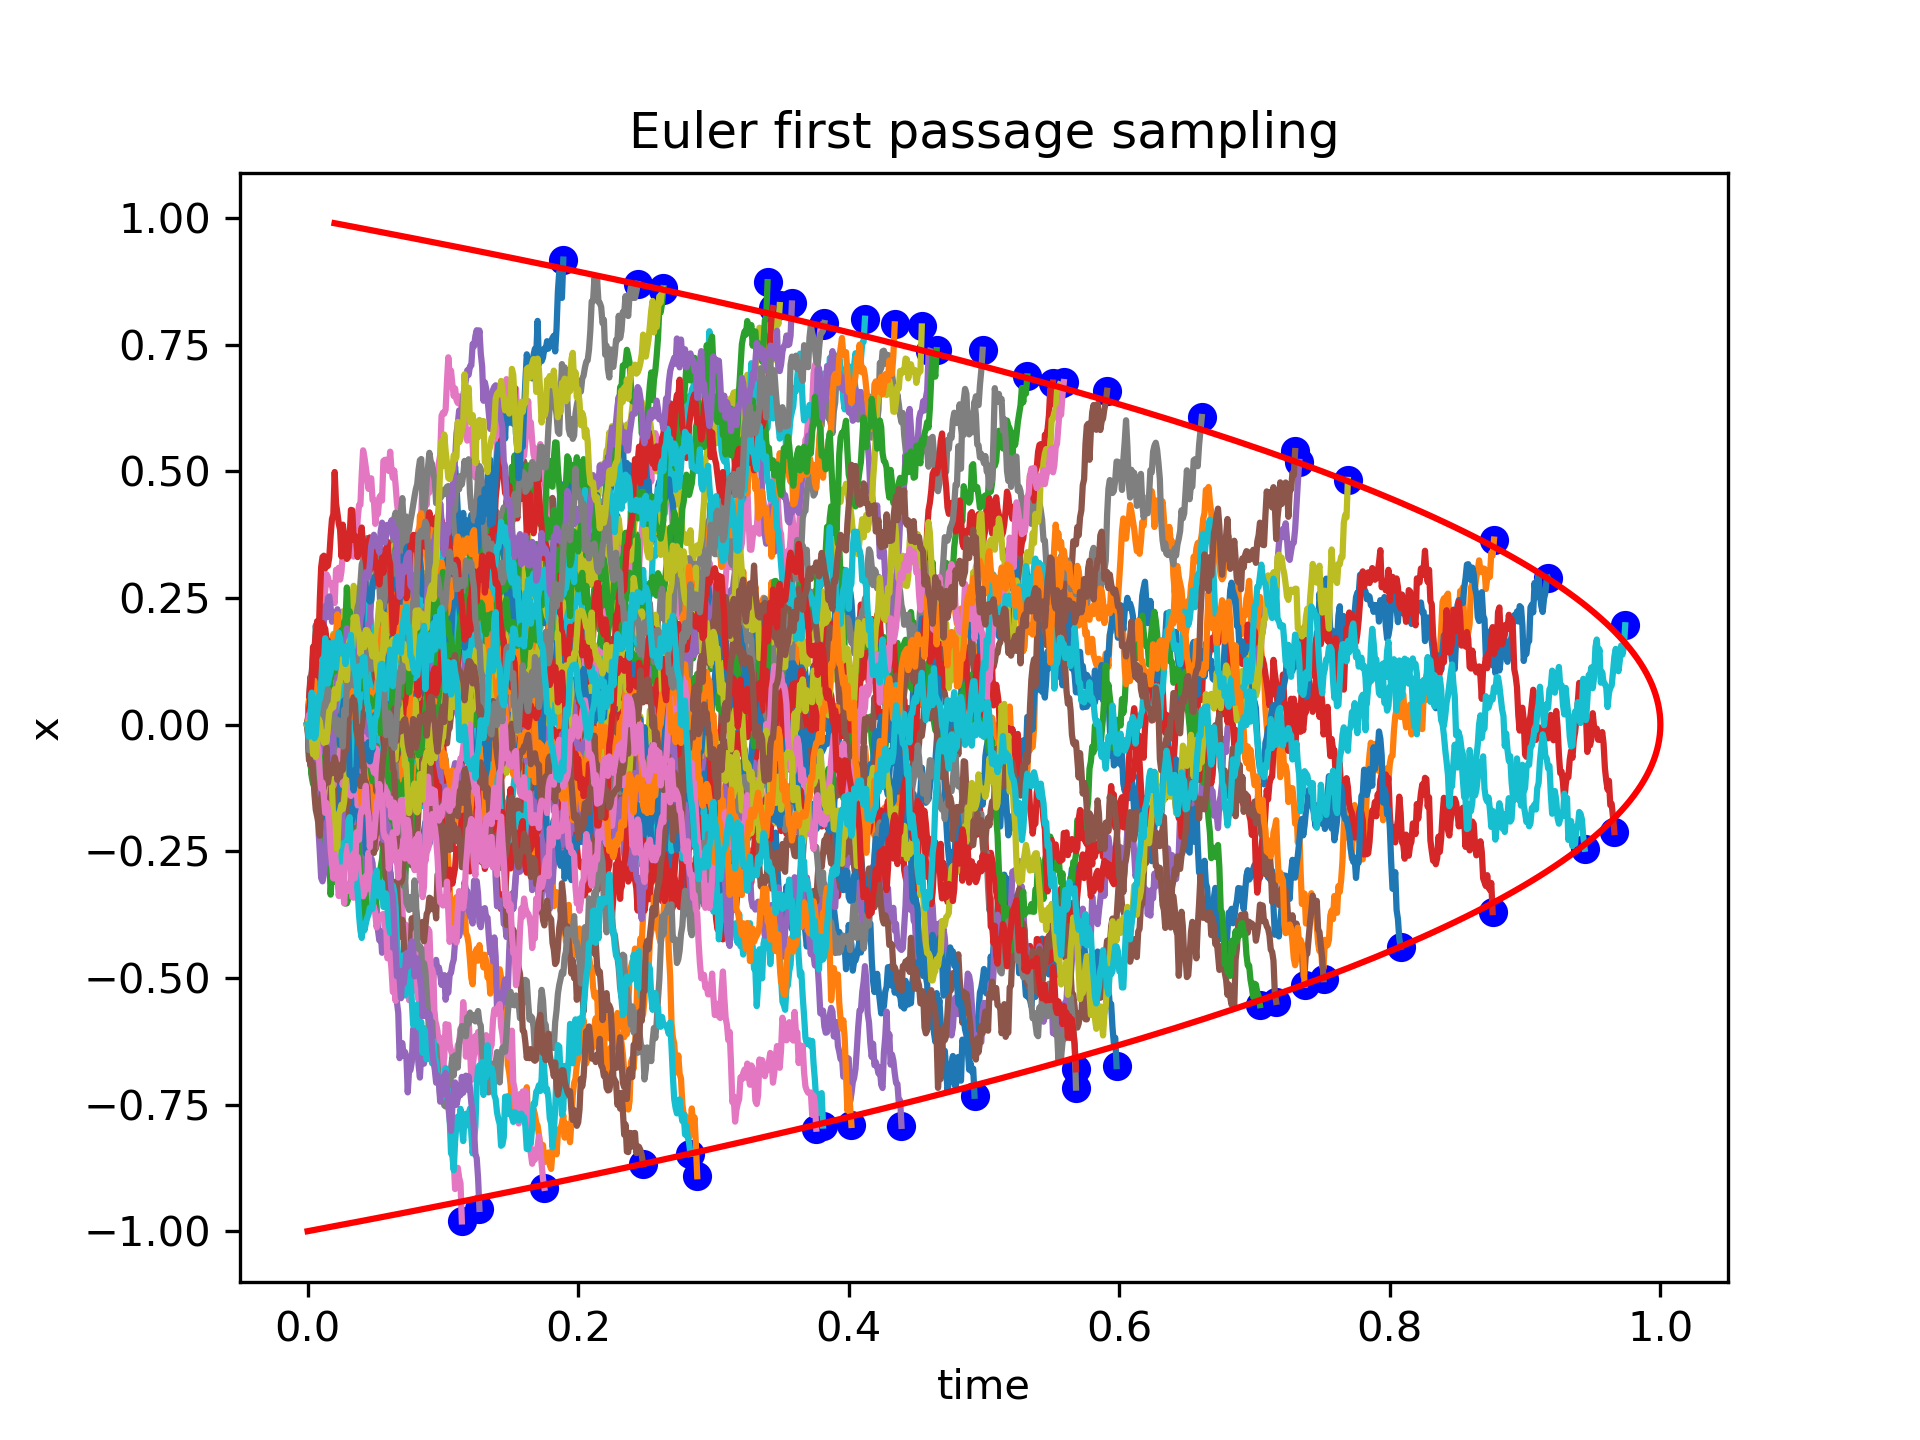
\includegraphics[width=0.8\textwidth]{plots/Euler first passage para.png}
        \caption{ $50$ realizations of Euler first passage sampling with step size $0.001$.}
        \label{fig:Euler first passage para}
    \end{figure}
\end{example}

\begin{lemma} \label{lem: FP order}
    When a process has more valid states the first passage time gets larger i.e.
    \begin{equation}
        V_{1} \subset V_{2} \Rightarrow
        \text{FPt}(X_{t}(\omega),V_{1}) \le  \text{FPt}(X_{t}(\omega),V_{2}) .
    \end{equation}
    The $\omega$ is to indicate we mean the same realization of $X_{t}$.
\end{lemma}


\begin{technique}[recursive first passage sampling]
    Recursive first passage sampling involves sampling an initial,
    simpler first passage, the base that includes fewer valid states. Using
    this sampled first passage as a starting point, we
    then perform the same sampling process until the sampled
    first passage is almost invalid.
\end{technique}


\begin{example}[recursive first passage sampling] \label{ex:recursive first passage sampling}
    In this example, we sample the first passage of Brownian motion from a parabolic barrier
    with recursive first passage sampling.
    For the simpler first passage sampler, we scale and translate
    samples from a triangular barrier so its
    valid states are contained in the parabola generated
    by the Euler scheme. The precomputed samples are created
    by (\ref{py:euler FP sampling}) and used to produce first passages
    in (\ref{py:recu FP sampling}).

\end{example}

\begin{pythonn}[Euler first passage sampling] \label{py:euler FP sampling}
    \pythoncode{python code/sample_euler_triangle.py}
\end{pythonn}

\begin{pythonn}[recursive first passage sampling] \label{py:recu FP sampling}
    The maximum scaling of the triangular barrier that fits
    in the parabola is derived through (\ref{lem:self affine})
    and using the fact that a parabola domain is convex. To dampen barrier
    overstepping of (\ref{py:euler FP sampling}) we use a smaller scaling
    than the maximum. \\
    \pythoncode{python code/sample_recu_para.py}

    \begin{figure}[h!]
        \centering
        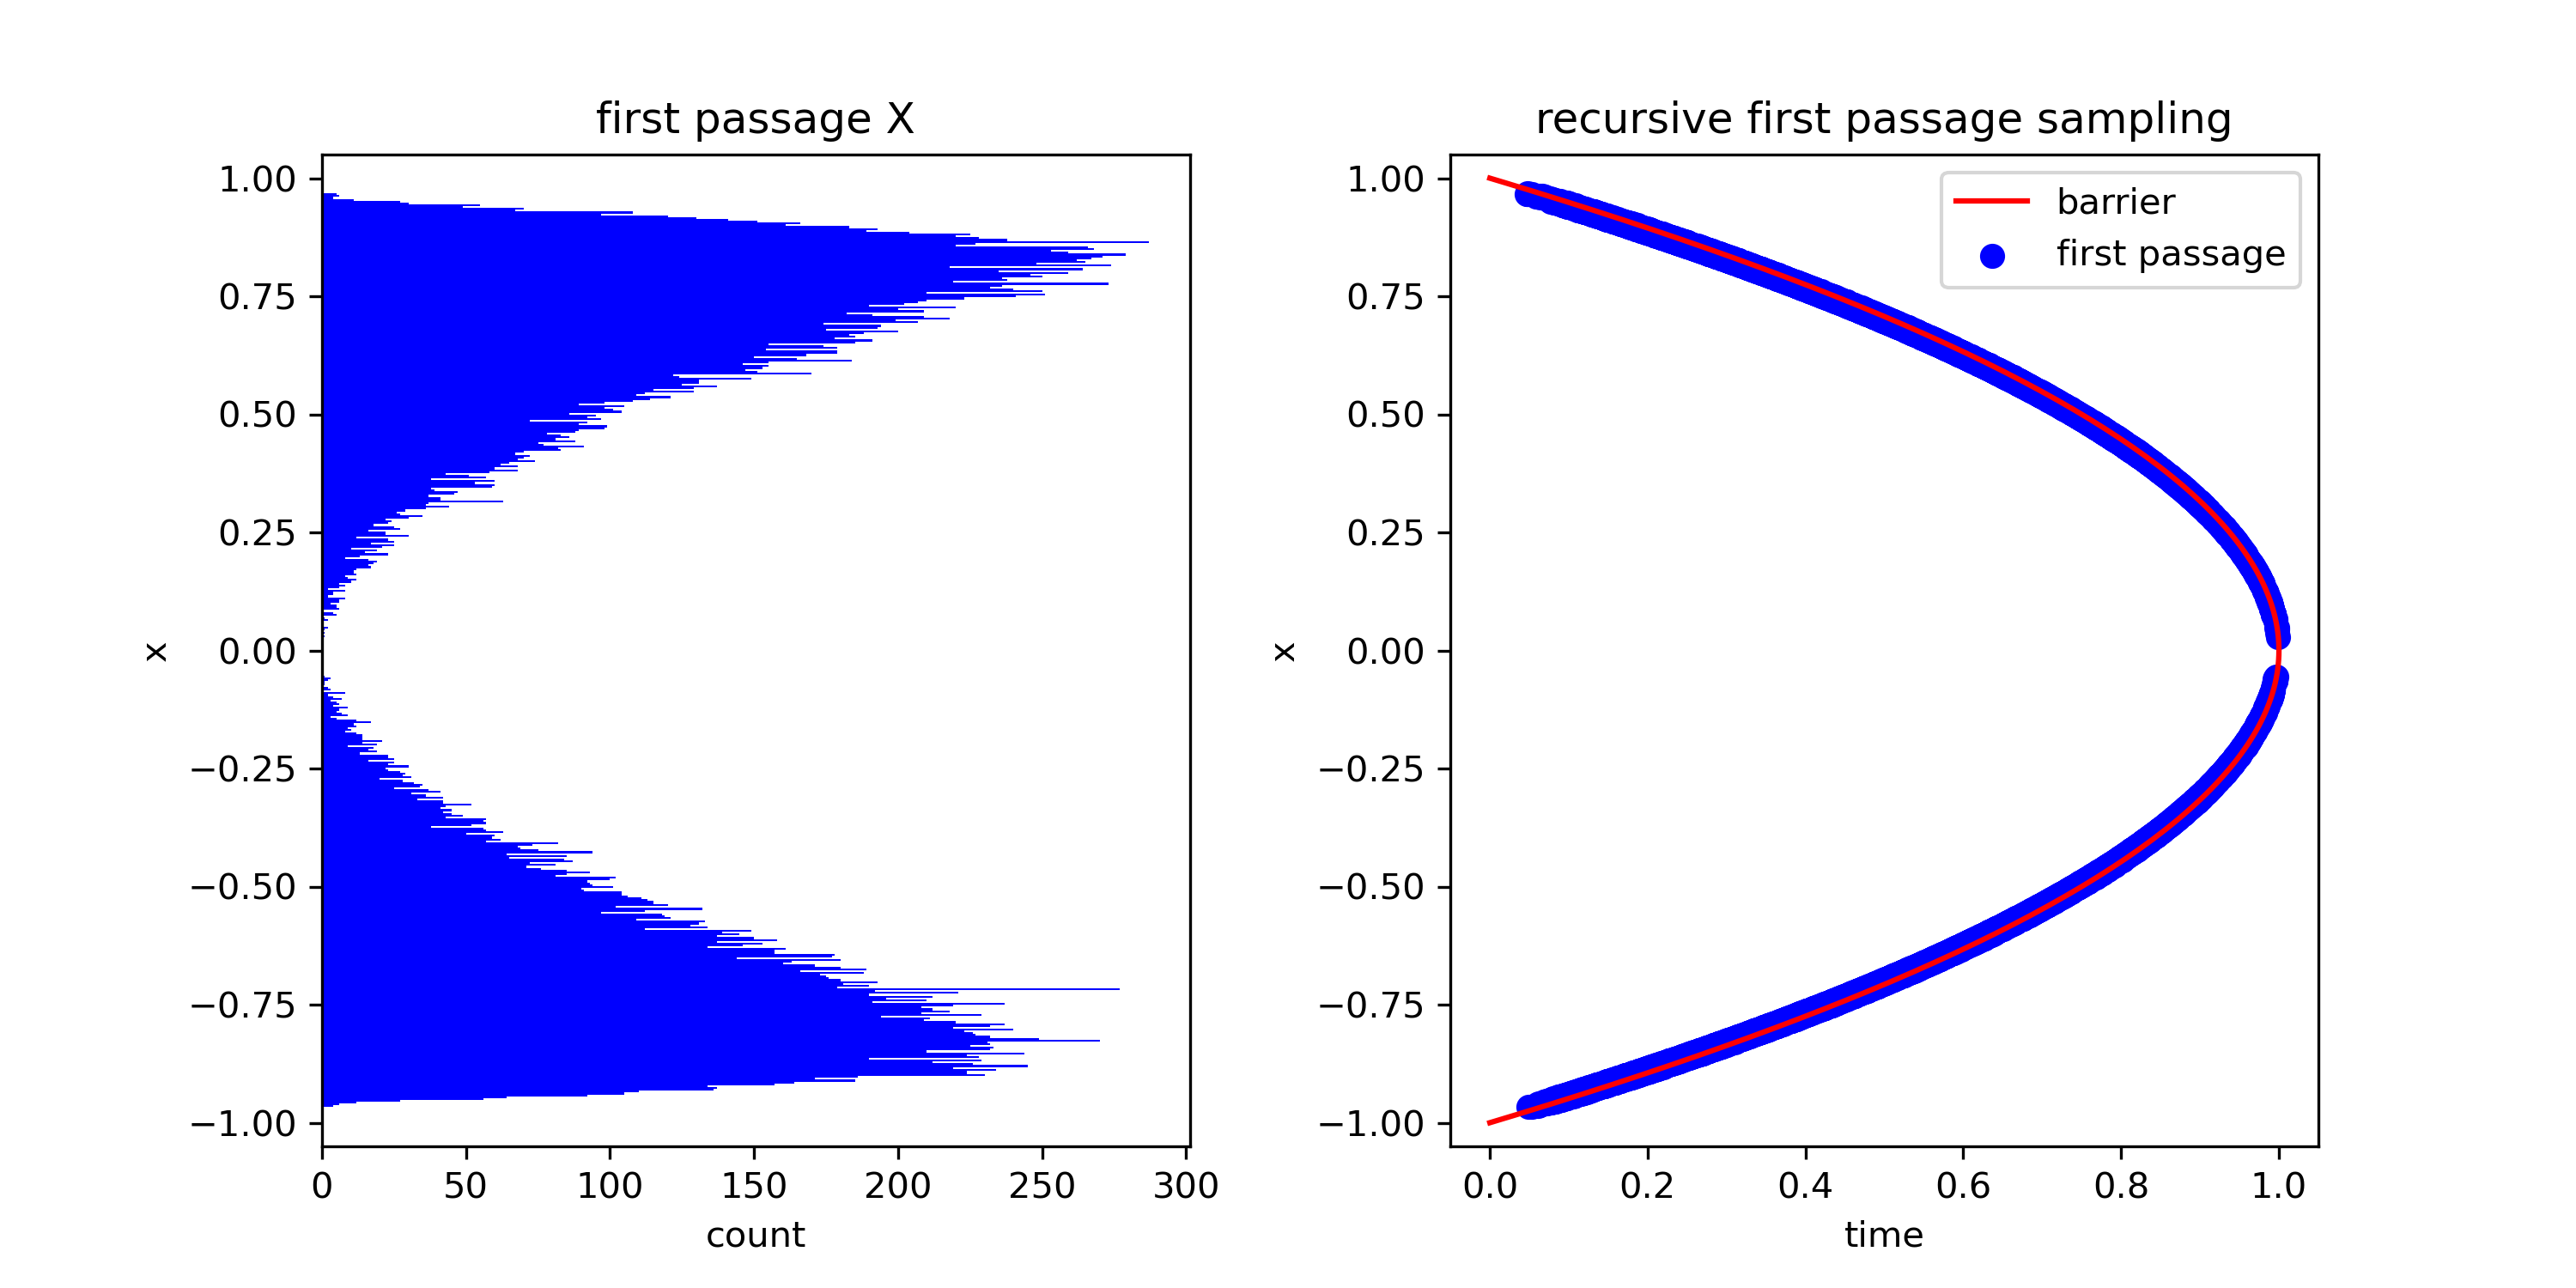
\includegraphics[width=1\textwidth]{plots/recursive first passage para.png}
        \caption{ $50000$ of realizations of recursive first passage sampling produced
            by (\ref{py:recu FP sampling}). The precomputed sample of $5000$ first
            passages of a triangular barrier uses the Euler scheme with
            step size $0.001$.}
        \label{fig:recursive first passage para}
    \end{figure}
\end{pythonn}

\begin{related}[recursive first passage sampling]
    The original walk on spheres is a recursive first passage algorithm.
    Recursive first passage sampling for
    Brownian motion is discussed in \cite{herrmann_first-passage_2016}
    and by transformation also first passage problems for the
    Ornstein-Uhlenbeck process.
    % To add jumps you can use \cite{herrmann_exact_2021}.
    An alternative to resampling from an Euler scheme is to use tabulated
    inverse cumulative probability functions,
    as demonstrated in \cite{hwang_simulationtabulation_2001}.
\end{related}

% For recursive first passage sampling for high dimensional Brownian motion
% there symmetry trick to be pulled off


\begin{example}[recursive first passage average sampling] \label{ex:recu FP average}
    In example (\ref{ex:recursive first passage sampling}) it is possible to keep
    track of the average because it scales and translates with our base first passage sampler.

    \begin{figure}[h!]
        \centering
        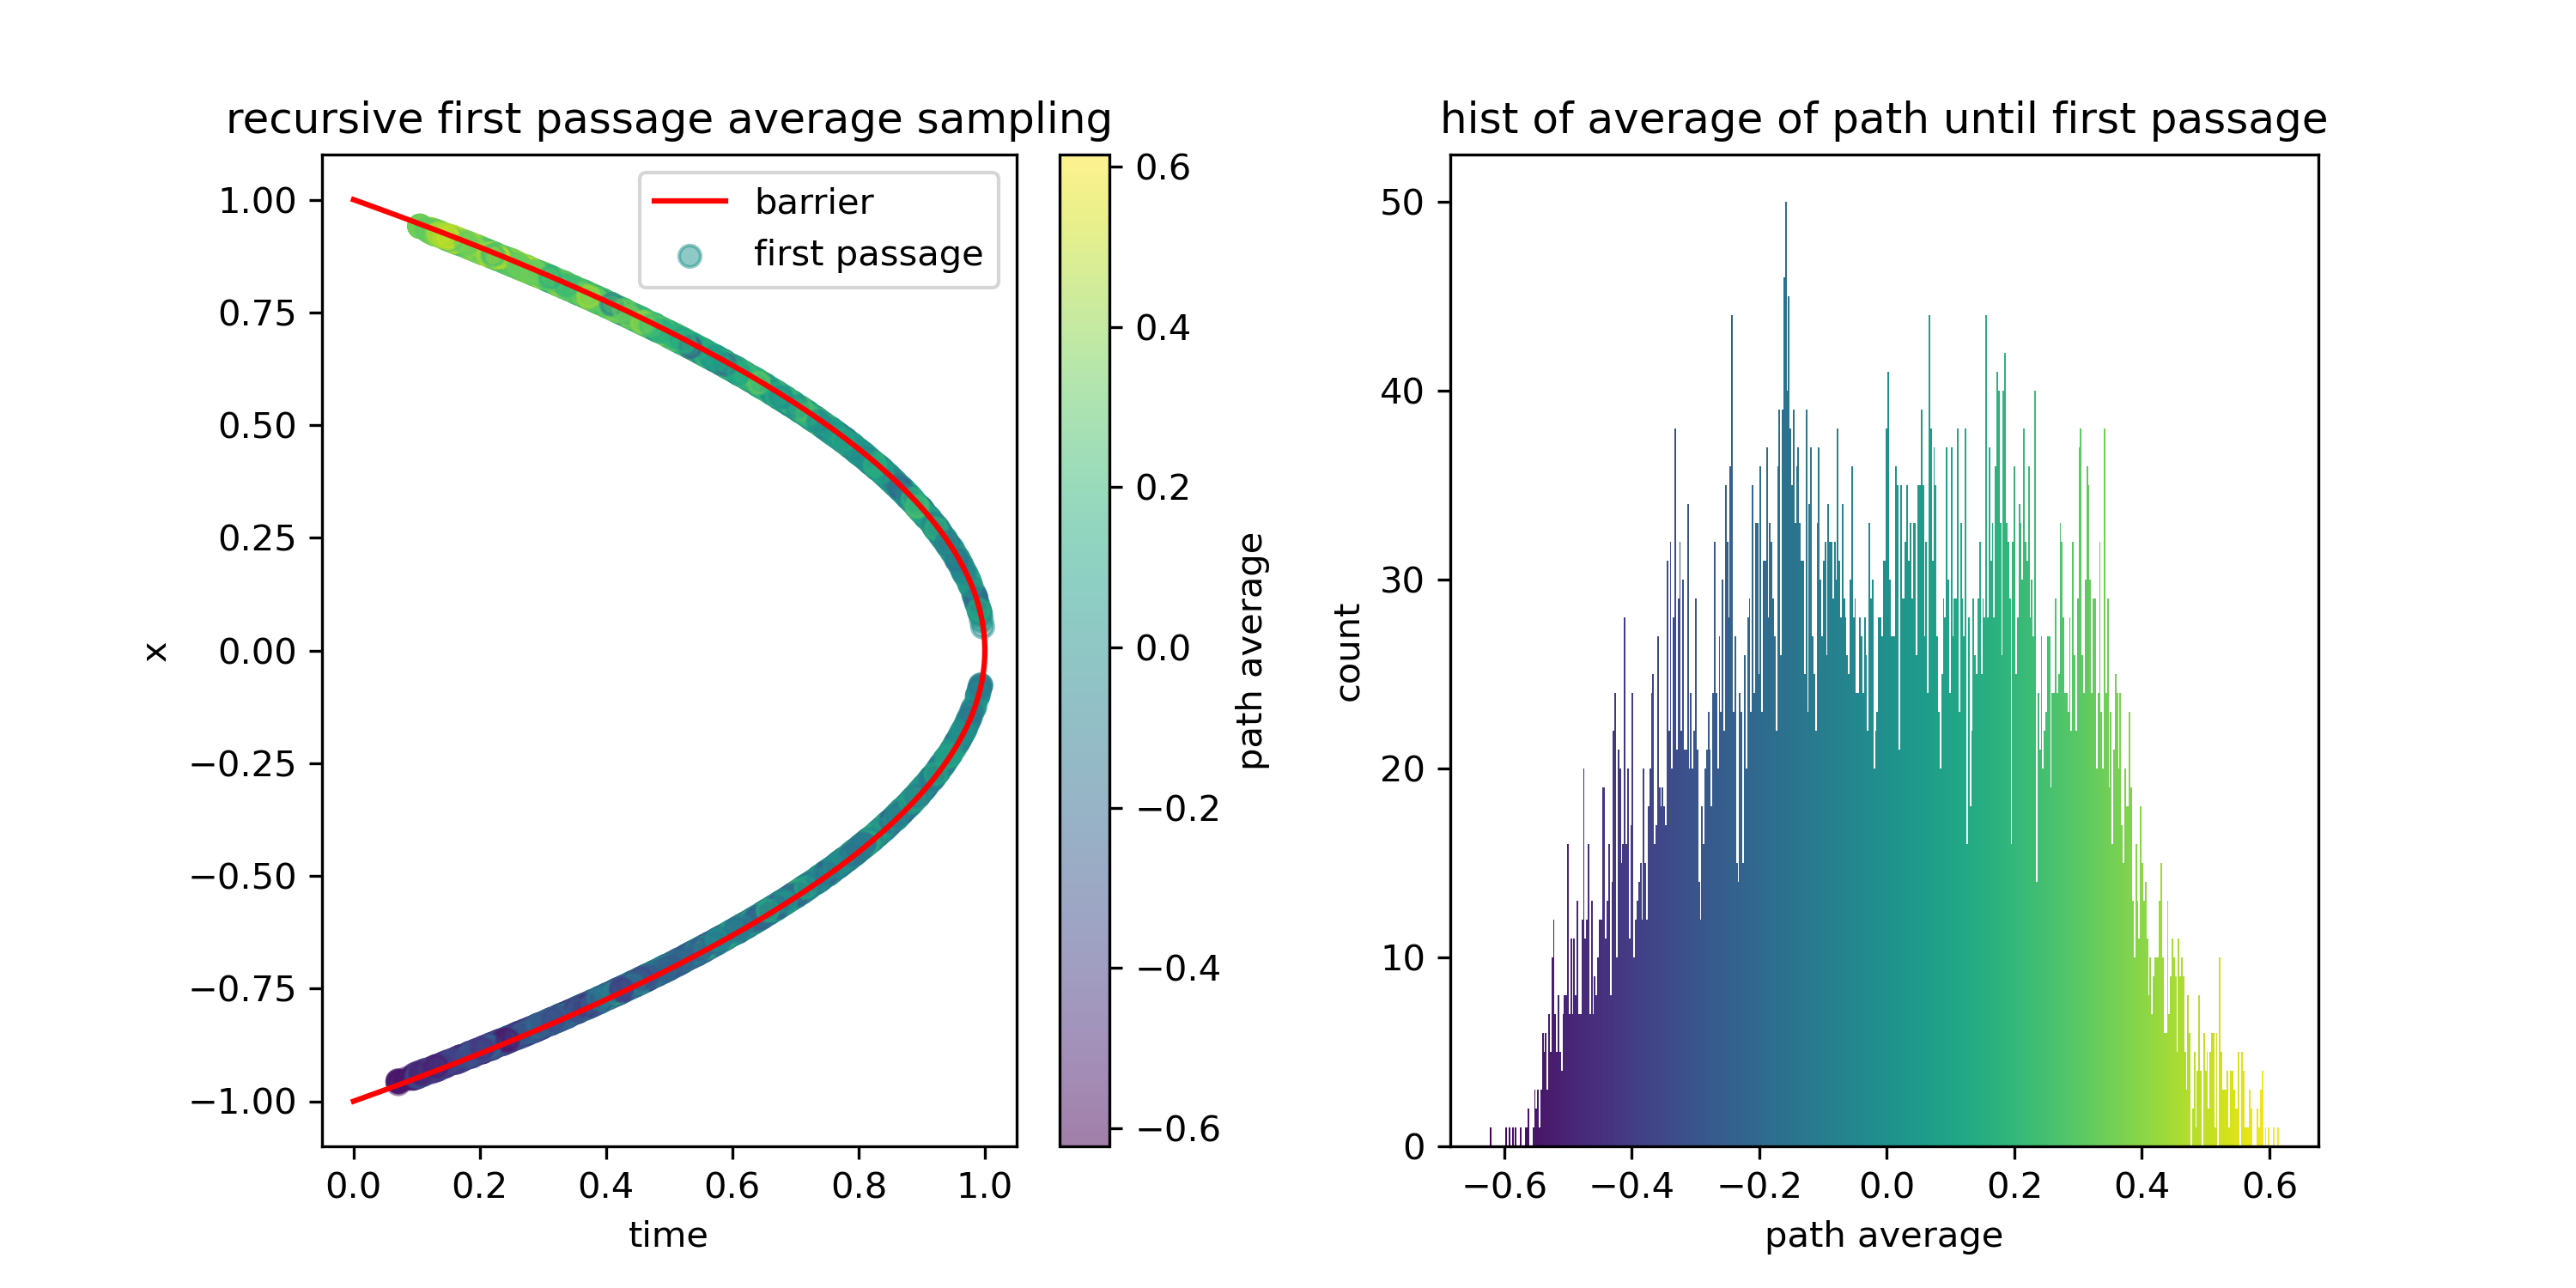
\includegraphics[width=1\textwidth]{plots/recursive first passage average para.png}
        \caption{ $10000$ of realizations of recursive first passage sampling (for the average).
            The precomputed sample of $1000$ first passages and averages of a triangular barrier
            uses the Euler scheme with step size $0.001$.}
        \label{fig:recursive first passage average para}
    \end{figure}
\end{example}


\begin{technique}[Brownian motion path stitching]
    Instead of thinking of sampling the first passages you can also sample
    whole paths to the first passage. Similar to before we need to be
    able to generate paths for a simple first passage problem and "stitch"
    these paths together. An advantage over normally generating paths
    is that a path can be represented by its subpaths and their scalings
    requiring less memory than a fully stored path. This can be useful
    in case you need to look back to a part of the path.
    The only downsides are that the time steps are inhomogeneous
    and it requires storing paths for the simpler first passage problem.
\end{technique}

\begin{example}[path stitching parabola]
    This is the same as example (\ref{ex:recursive first passage sampling}) but now we have
    to keep track of the whole resampled Euler scheme generated paths.

    \begin{figure}[h!]
        \centering
        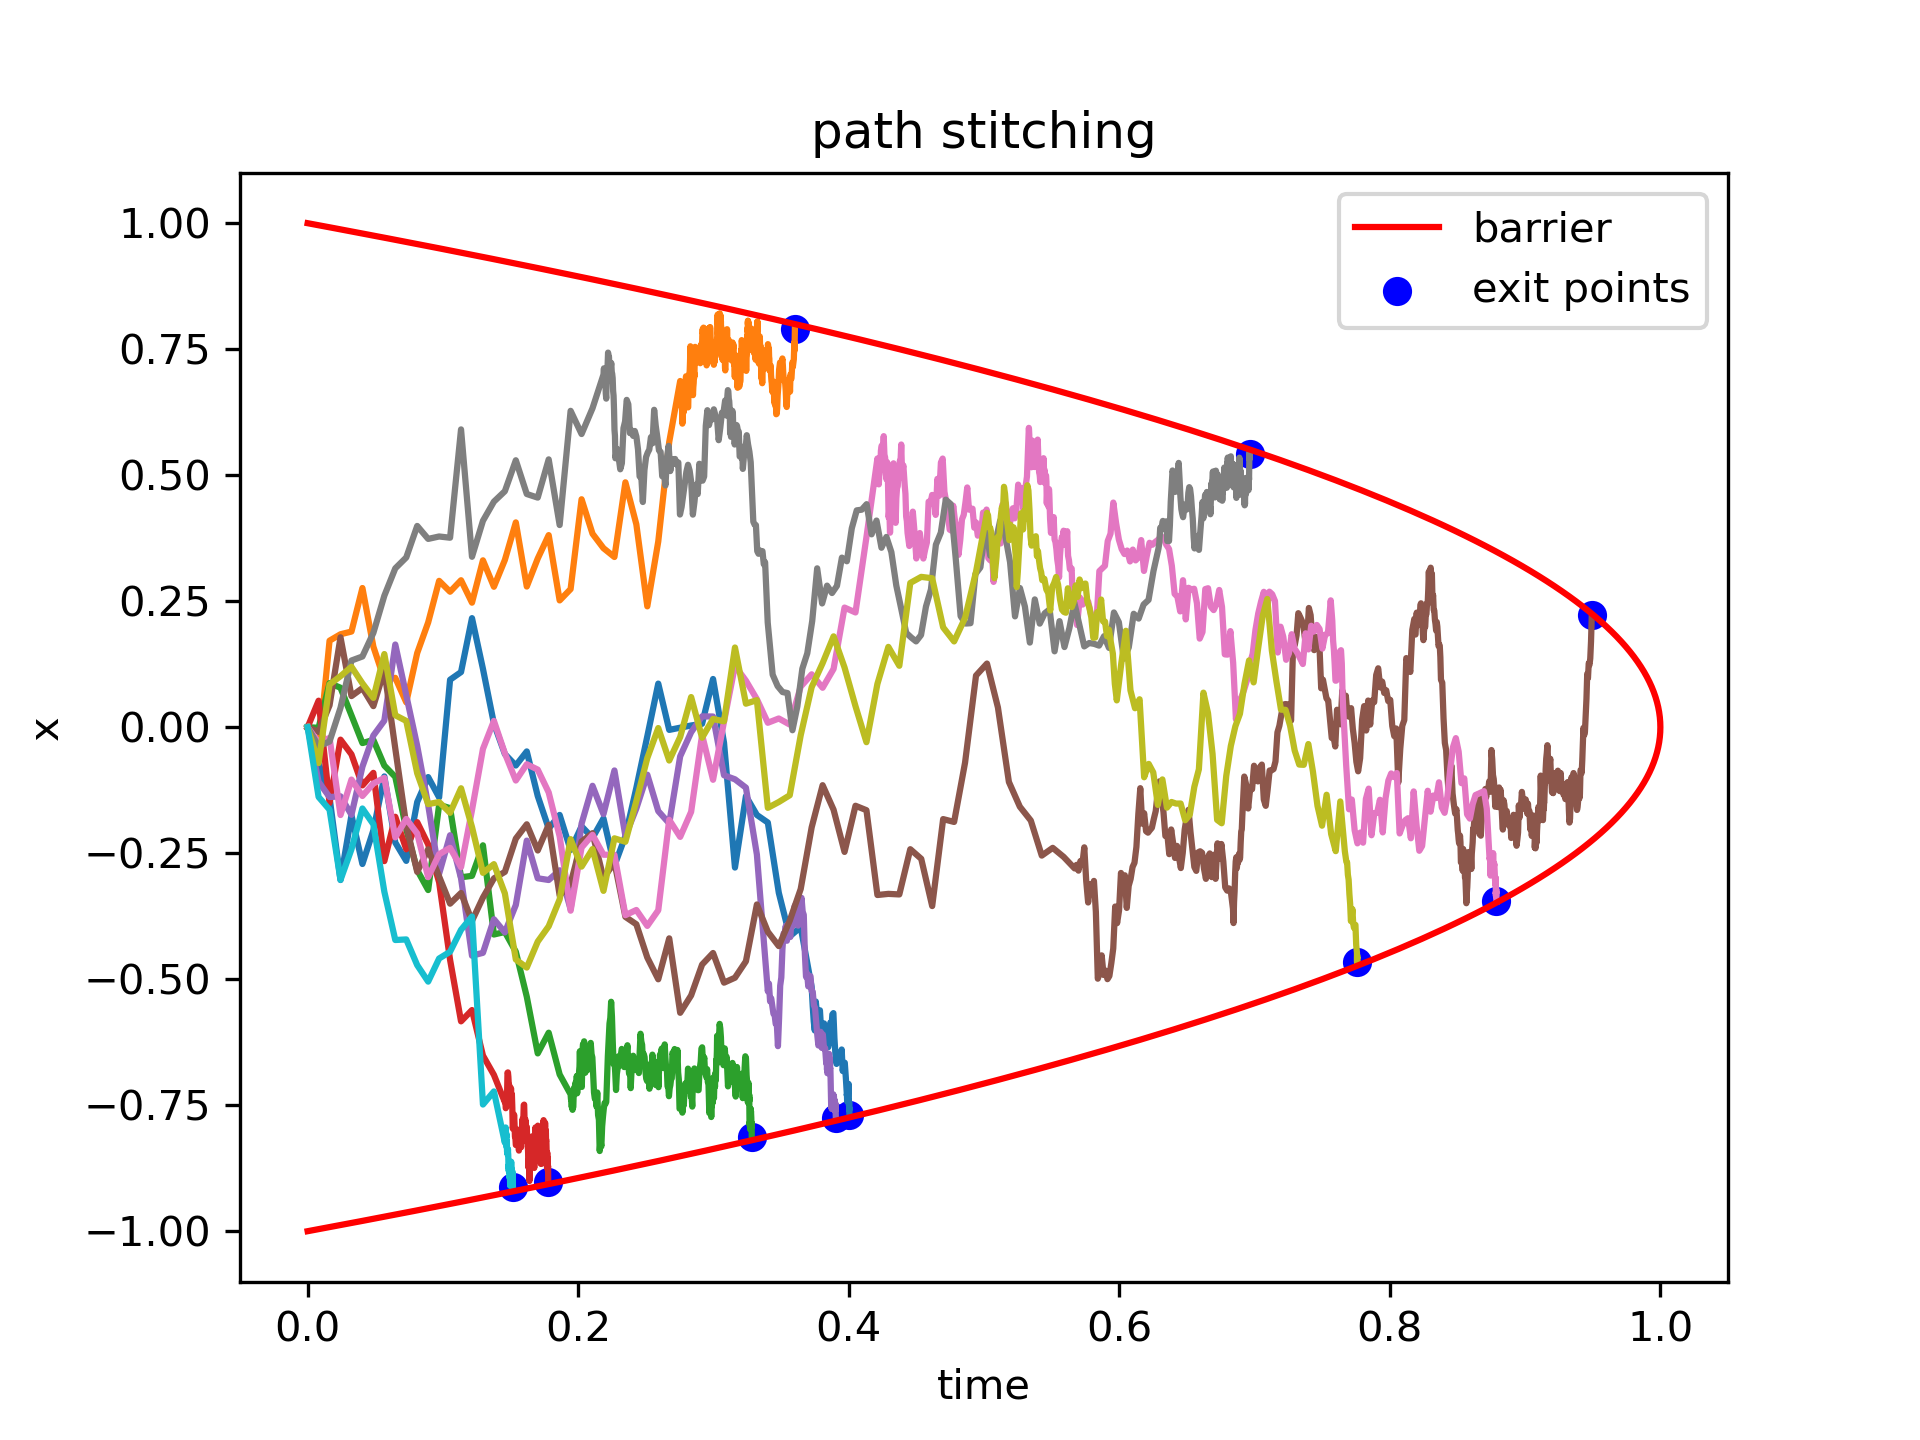
\includegraphics[width=0.8\textwidth]{plots/path stitching para.png}
        \caption{ $10$ paths build with path stitching build out of
            precomputed Euler scheme generated paths with step size $0.01$.}
        \label{fig:path stitching para}
    \end{figure}
\end{example}

% For plotting the path we needed to accesses to all of its points.  

% A way around scaling base samples is limiting scaling to a
% discrete set and pick the biggest scaling that fits, instead
% of generating base samples for $1$ scale and scaling it dynamically
% precompute all the discrete scalings. \\


\begin{related}[path stitching]
    Path stitching appears frequently in rendering and also in \cite{das_sarma_fast_2015}
    and \cite{ji_reusing_2012}.
\end{related}

\subsection{Limitations and Future Work}

It would be interesting to extend proof technique of (\ref{lem:BM HE}) to the full
Feynman-Kac formula. Just adding a source term $f$ in the Feynman-Kac formula adds
an integral of the source term over the recursion path.
In equation (\ref{eq:discrete iso heat equation})
it would add $\frac{\Delta t \Delta x^{2}}{2 \Delta t + \Delta x ^{2}} f(x,t)$
term. This term can either be kept or Russian rouletted
to prevent infinite source evaluations in the limit.
This roughly corresponds to estimating the integral by
MC integration also requires knowing a finite amount of
intermediate points of the recursion path
sampled randomly. These can possibly be obtained from
the intermediate first passages of recursive first passage sampling or with a smart
application of path stitching. \\


Recursive first passage sampling for Brownian motion can be extended to geometric
Brownian motion by transforming the space. However, this transformation breaks
the symmetries required for the average used in the example (\ref{ex:recu FP average}).
An unsatisfying way to fix this is to approximate the base sampler at different points in
space and at different scales. Just accelerating a classic Euler scheme at critical places
with a base sampler can reduce precomputation requirements.


\newpage
% \selectlanguage{Dutch}
\begin{abstract}
    Deze scriptie onderzoekt unbiased Monte Carlo methoden voor
het oplossen van lineaire gewone differentiaalvergelijkingen met het
oog op partiële differentiaalvergelijkingen.
De voorgestelde algoritmes maken gebruik van de geschikte
combinatie van Monte Carlo technieken. Deze Monte Carlo technieken
worden geïntroduceerd met voorbeelden en code.
\end{abstract}

% \selectlanguage{English}
\printbibliography
\newpage

% \section{Appendix}
% Derivation of the green functions and some expressions.
\end{document}
